\documentclass[12pt]{article}
\usepackage[utf8]{inputenc}
\usepackage[dutch]{babel}
\usepackage[rightcaption]{sidecap}
% \usepackage{minted}
\usepackage{graphicx}
\usepackage[colorlinks=true, allcolors=blue]{hyperref}
\usepackage{sectsty}
\usepackage[paperheight=29.7cm,paperwidth=21cm,textwidth=15cm]{geometry} %A4 size
\usepackage{fancyhdr}
\usepackage[siunitx]{circuitikz}
\usepackage{tabularx}
\usepackage{physunits}
\usepackage{booktabs}
\usepackage{tikz}
\usepackage{pgfplots}
\usepackage{karnaugh-map}
\usepackage[nocompress]{cite}
\usepackage{cite}
\usepackage{parskip}
\usepackage{amsmath,amssymb,amsfonts}
\usepackage{algorithmic}

% The preceding line is only needed to identify funding in the first footnote. If that is unneeded, please comment it out.
\usepackage{textcomp}
 % More defined colors
% We will externalize the figures



% Footers/Headers opmaak:
\pagestyle{fancy}
\lhead{}
\chead{\textit{Practicum 5: Digitale Techniek - Asynchrone tellers
}}
\rhead{}
\lfoot{\textit{Semih Can Karakoç}}
\cfoot{\textit{\today}}
\rfoot{\textit{\thepage}}
\renewcommand{\headrulewidth}{0.1pt}
\renewcommand{\footrulewidth}{0.4pt}

% Afbeelding settings:
\graphicspath{ {./Figures/} }
% \sectionfont{\left}
% \subsectionfont{\centering}
% \subsubsectionfont{\centering}

% Voorpagina opmaak:
\title{\textbf{Practicum 5: Digitale Techniek - Asynchrone tellers}}
\author{\textit{Semih Can Karakoç (695258)}}
\date{\textit{\today}}

% Begin document
\begin{document}

\clearpage\maketitle    % Pas opmaak toe aan voorpagina
\thispagestyle{empty}  % Haal page number weg
% Voorpagina plaatje:
\begin{figure}[h]
    \centering
    % \includegraphics[width=0.6\textwidth]{ELEKTRA.png}
\end{figure}
\pagebreak

\tableofcontents    % Inhoudsopgave
\pagebreak

\section{Inleiding}
Tijdens dit practicum is er geëxperimenteerd en onderzocht naar de werking van de modulo-16 teller en de decade teller.
Het doel van dit laatste practicum is dan ook om de aspecten van deze logische functies te begrijpen en in de praktijk toe te kunnen passen.
Om de bovenstaande practicumdoel te behalen zijn er twee practicumexperimenten uitgevoerd. 
Daarbij zijn de bijbehorende deelopdrachten uitgewerkt in dit verslag. 

Dit verslag gaat in op de volgende onderwerpen: 
\begin{enumerate}
    \item Logische schakelingen lezen, bouwen en ontwerpen;
    \item Decade teller;
    \item Modulo-16 teller;
    \item J-K-flip-flop;
    \item Waarheidstabellen;
    \item Asynchrone tellers;
    \item Schmitt-trigger;
    \item Booleaanse algebra.
\end{enumerate}
\vspace{8cm}
NOTE: \textit{alle getekende logische schakelingen in dit verslag zijn zelf gemaakt met draw.io!}
\pagebreak
\section{Probleem- en doelstelling}
\label{Problem}
Dit verslag bevat de volgende probleemstelling:
\begin{itemize}
    \item \textit{``Hoe kunnen J-K-flip-flops worden toegepast bij het ontwerpen en bouwen van asynchrone tellers?''}
\end{itemize}
\vspace{0,5cm}
De volgende doelstellingen behoren tot dit practicum:
\begin{enumerate}
    \item Inzicht te verkrijgen in logische functies die ten grondslag liggen aan de digitale techniek;
    \item Waarnemingen te verrichten aan de bijbehorende eenvoudige logische schakelingen;
    \item De bijbehorende meetgegevens en waarheidstabellen op een juiste wijze te verkrijgen en te interpreteren;
    \item De vergaarde gegevens te verwerken tot een verslag.
\end{enumerate}

\vspace{0,5cm}
Aan het einde van dit verslag onder het kopje \ref{Conclusie}:\textit{``Conclusie''} zal de gestelde probleemstelling beantwoord worden.
\pagebreak

\section{Practicumbenodigdheden}
\label{practicumbenodigdheden}
Hieronder zijn de benodigdheden op een rijtje gezet die nodig waren voor het uitvoeren van het practicum:
\begin{enumerate}
    \item Digiboard: het 3910 digiboard is een bord waarop je gemakkelijk de logische schakelingen kan bouwen door gebruik te maken van de ingebouwde poorten. Deze hebben we gebruikt tijdens het practicum.\cite{hps-systemtechnik_ds_DIGI};
    \item Verbindingssnoeren: deze snoeren zijn nodig om verbinding te maken tussen allerlei elektronische componenten; 
    \item Draw.io: dit is een online website waarmee je gemakkelijk logische schakelingen kunt ontwerpen;
\end{enumerate}
\pagebreak

\section{Theoretisch kader}
\label{Theoretisch kader}
\subsection{De basispoorten}
In de digitale techniek zijn er drie belangrijke basispoorten, namelijk:
\begin{enumerate}
    \item De AND-poort: de AND-poort voert een vermenigvuldiging uit tussen de inputs. Dit betekent dat de AND-poort alleen `1' terug geeft wanneer de alle inputs ook `1' zijn, want een vermenigvuldiging met '0' geeft altijd '0' terug. Dit wordt uitgedrukt als: $A \cdot B$;
    \item De OR-poort: de OR-poort voert een optelling uit tussen de inputs. Dit betekent dat de OR-poort alleen `1' terug geeft wanneer minimaal een van de twee inputs `1' is, want een optelling met '1' en '0' is altijd '1'. Dit kan worden uitgedrukt als: $A + B$;
    \item De NOT-poort: de NOT-poort voert een inversie uit op de input. Dit betekent dat de NOT-poort altijd het tegenovergestelde van de input terug zal geven. Een voorbeeld is: $A$ wordt $\overline{A}$ (A niet) \cite{electricalengineering123}.
\end{enumerate}
\subsection{Waarheidstabellen}
Tijdens het practicum wordt ook gebruik gemaakt van waarheidstabellen. 
Een waarheidstabel is een tabel die overzicht geeft over alle mogelijke combinaties van inputwaarden en de bijbehorende uitvoerwaarden \cite{truth2}. 
De waarheidstabel begint aan de linkerkant met de inputwaarden. 
Nadat alle inputwaarden zijn genoteerd komen er twee verticale strepen. 
Deze twee strepen geven aan dat de daarop volgende variabelen uitvoerwaarden zijn \cite{truth1}.  

Zie hieronder een voorbeeld van een waarheidstabel die twee inputwaarden heeft: `A' en `B', en één uitvoerwaarde heeft, namelijk: `$A \cdot B$' (AND-operatie). 
Met deze waarheidstabel kun je alle mogelijkheden overzichtelijk terug zien.
\begin{displaymath}
    \begin{array}{|c|c||c|}
    A & B & A \cdot B \\
    \hline 
    1 & 1 & 1 \\
    1 & 0 & 0 \\
    0 & 1 & 0 \\
    0 & 0 & 0
    \end{array}
    \end{displaymath}
\pagebreak
\subsection{Wetten van de Booleaanse algebra}
In de Booleaanse algebra zijn er een aantal belangrijke wetten die je kunt toepassen om Booleaanse expressies te kunnen vereenvoudigen, namelijk:
\begin{itemize}
    \item Associativiteit: $A+(B+C) = (A+B)+C$ en $A\cdot(B\cdot C) = (A\cdot B)\cdot C$; 
    \item Commutativiteit: $A+B = B+A$ en $A\cdot B = B\cdot A$;
    \item Absorptie: $A+(A\cdot B) = A$ en $A \cdot (A+B) = A$;
    \item Complement: $A + \overline{A} = 1$ en $A \cdot \overline{A} = 0$;
    \item Distributiviteit: $A+(B\cdot C) = (A+B)\cdot (A+C)$ en $A \cdot (B+C) = (A\cdot B)+(A\cdot C)$;
    \item Idempotentie: $A + A = A$ en $A \cdot A  = A$;
    \item De Morgan: $\overline{A \cdot B} = \overline{A}+\overline{B}$ en $\overline{A + B} = \overline{A} \cdot \overline{B}$;
    \item Redundantie: $A\cdot B + A\cdot \overline{B} = A$ en $A\cdot \overline{B} + B = A + B$
    \item Dubbele negatie: $\overline{\overline{A}} = A$ \cite{weyt}.
\end{itemize}
\pagebreak
\subsection{Schmitt-trigger}
Een ``Schmitt-trigger'' is een comparator met twee spanning-thresholds, namelijk: de bovenste spanning-threshold ($V+$) en de onderste spanning-threshold ($V-$). 
Hieronder staat een lijst met de mogelijke trigger-toestanden:
\begin{itemize}
    \item Wanneer $V_{in}$ de bovenste spanning-threshold overschrijdt dan zal de Schmitt-trigger een hoog signaal geven;
    \item Wanneer $V_{in}$ de onderste spanning-threshold overschrijdt dan zal de Schmitt-trigger nog niets doen;
    \item Wanneer $V_{in}$ zakt onder de onderste spanning-threshold dan zal de Schmitt-trigger een laag signaal geven \cite{schmit}. 
\end{itemize}
Dit betekent dat de Schmitt-trigger een hoog signaal zal geven wanneer de spanningswaarde de bovenste threshold overschrijdt en een laag signaal geven wanneer die spanningswaarde weer onder de onderste threshold komt. 
Zie het figuur hieronder waarbij er een Schmitt-trigger is toegepast. In de figuur representeert de groene stippellijn de bovenste spanning-threshold ($V+$) en de rode stippellijn de onderste spanning-threshold ($V-$):
\begin{figure}[h]
    \begin{minipage}{.5\textwidth}
    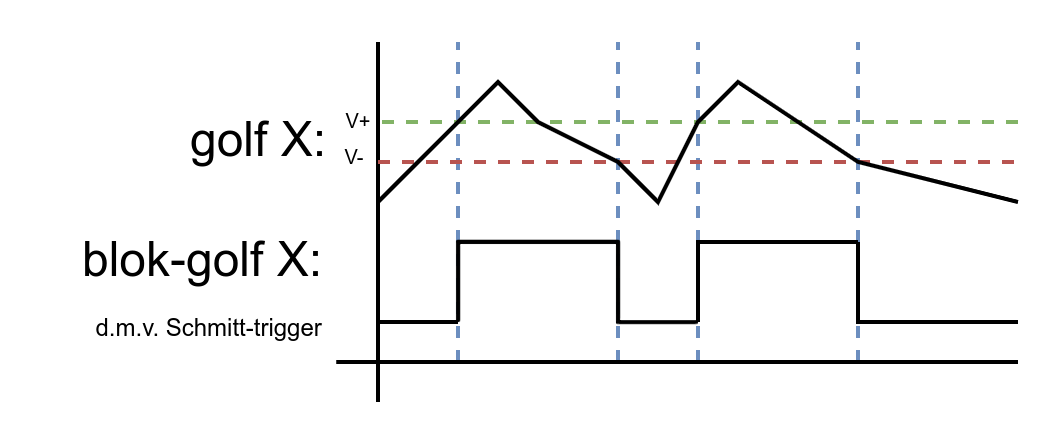
\includegraphics[width=1\textwidth]{schmitt.png}
    \caption{Schema waarin te zien is dat golf $X$ omgezet wordt in een blokjesgolf d.m.v. een Schmitt-trigger.}
    \label{fig:39100}
\end{minipage}
\begin{minipage}{0.5\textwidth}
    
\includegraphics[width=1\textwidth]{st.png}
    \caption{Schmitt-trigger symbool}
    \label{fig:39910}
\end{minipage}
\end{figure}\\
Tijdens dit practicum wordt de geïnverteerde Schmitt-trigger toegepast in de logische schakeling van de decade-teller. 
De decade-teller is een binaire teller dat van 0 tot en met 9 telt en cyclisch dit blijft herhalen. 
Als we in dat logische circuit geen geïnverteerde Schmitt-trigger zouden gebruiken, springt de decade-teller van 9 naar 2 en worden 0 en 1 overgeslagen.  
Dit komt door onstabiele overgangen in de signalen van de gebruikte logische poorten. 
Logische poorten hebben een maximale stijg en val tijd voor de input, wanneer deze te hoog wordt, kunnen er zulke onstabiele overgangen in signalen ontstaan.
% \subsection{Karnaugh diagram}
% In de Booleaanse algebra moet je vaak een SOP (Sum Of Products) of een POS-expressie (Product Of Sum) opstellen. Deze expressies zijn meestal nog niet vereenvoudigd tot een minimale expressie. 
% Het minimaliseren van een SOP of een POS-expressie kan efficiënte logische schakelingen opleveren, omdat er dan minder logische poorten nodig zijn om dezelfde output te verkrijgen \cite{Karnaugh1953}. 
% Dit is mogelijk door het gebruik van Karnaugh diagrammen. Een Karnaugh diagram (afgekort K-map) bestaat meestal uit een 2x2, 2x4 of 4x4 raster, echter is dit afhankelijk van hoeveel variabelen je hebt. 
% Stel dat we de volgende variabelen hebben: $A, B, C, D$, dan wordt het volgende gedaan:
% \begin{enumerate}
%     \item Eerst maken we twee groepen met twee variabelen: $G_{1} = AB$ en $G_{2} = CD$;
%     \item Aangezien we vier variabelen ($ABCD$) hebben, krijgt de K-map een 4x4 raster;
%     \item Groep 1 zetten we aan de linkerkant van de K-map en groep 2 zetten we aan de bovenkant van de K-map;
%     \item Nu beginnen we voor beide groepen linksboven met de volgende bits: 00. Voor groep 1 wordt de eerst volgende stap naar beneden toe geschreven. Voor groep 2 wordt de eerst volgende stap naar rechts toe geschreven. De stappen van groep 1 en 2 worden op deze manier verder uitgewerkt. De uitbreiding in het raster is als volgt: 00, 01, 11 en tenslotte 10;
%     \item Nu kunnen we de SOP-expressie invullen in de K-map en groepjes maken van 2, 4, 8, 16 (machten van 2) waar een vakje in het raster een `1' bevat;
%     \item Alle `1' in de K-map moet minimaal een groepje hebben, en het doel is om zo groot mogelijke groepjes te maken wat leidt tot de beste vereenvoudiging;
%     \item Tenslotte kijk je naar de groepjes (edge-edge mag ook) en moeten de variabelen dezelfde waarde hebben, anders neem je die variabele niet mee in je vereenvoudigde expressie (zie voorbeeld K-map hieronder).
% \end{enumerate} 
% \begin{center}
%         \begin{karnaugh-map}(label=corner)[4][4][1][$D$][$C$][$B$][$A$]
%             \manualterms{1,1,1,1,1,1,1,1,1,1,1,1,1,1,1,1}
%             \implicant{0}{2}
%             \implicant{5}{15}
%             \implicantedge{1}{3}{9}{11}
%             \implicantcorner
%             \implicantedge{4}{12}{6}{14}
%         \end{karnaugh-map}
% \end{center}

% Om het nog iets duidelijker te maken is hieronder nog een voorbeeld uitgewerkt.
% Gegeven is de volgende SOP-expressie: $\overline{A}\ \overline{B}\ \overline{C}\ \overline{D} + \overline{A}\ B\ \overline{C}\ \overline{D} + \overline{A}\ B\ C\ D + \overline{A}\ \overline{B}\ C\ D + \overline{A}\ B\ C\ \overline{D} + A\ \overline{B}\ C\ D$. 
% \begin{center}
%     \begin{karnaugh-map}(label=corner)[4][4][1][$D$][$C$][$B$][$A$]
%         \manualterms{1,0,0,1,1,0,1,1,0,0,0,1,0,0,0,0}
%         \implicant{7}{6}
%         \implicantedge{3}{3}{11}{11}
%         \implicant{0}{4}
%     \end{karnaugh-map}
% \end{center}
% In het gele vak zien we dat A allebei `0' is, we zien ook dat B zowel een `1' als een `0' heeft, dus B nemen we niet mee. Dan krijgen we: $\overline{A}\ \overline{C}\ \overline{D
% }$. 
% In het rode vak zien we dat C allebei `1' is, we zien ook dat D zowel een `1' als een `0' heeft, dus D nemen we niet mee. Dan krijgen we: $\overline{A}\ \overline{B}\ \overline{C} + \overline{A}\ B\ C$. 
% In het groene vak zien we dat B allebei `0' is, we zien ook dat A zowel een `1' als een `0' heeft, dus A nemen we niet mee. Tenslotte krijgen we de geminimaliseerde SOP: $\overline{A}\ \overline{C}\ \overline{D} + \overline{A}\ B\ C + \overline{B}\ C\ D$.
\pagebreak
\subsection{7-segmentdisplay}
Een 7-segmentdisplay is een display dat bestaat uit zeven lijnvormige segmenten die samen een 8 vormen. 
De segmenten zijn gelabeld van `a' tot en met `g', zie afbeelding \ref{fig:39110}. 
Door deze segmenten op een unieke manier aan en uit te zetten, is het mogelijk om elk getal van 0 tot en met 9 te representeren op het display \cite{7seg}. 
\begin{itemize}
    \item Het getal 0 is te representeren met segmenten: $a,b,c,d,e,f$;
    \item Het getal 1 is te representeren met segmenten: $b\ \&\ c$;
    \item Het getal 2 is te representeren met segmenten: $a,b,g,e,d$;
    \item Het getal 3 is te representeren met segmenten: $a,b,g,c,d$;
    \item Het getal 4 is te representeren met segmenten: $b,c,f,g$;
    \item Het getal 5 is te representeren met segmenten: $a,c,d,f,g$;
    \item Het getal 6 is te representeren met segmenten: $a,c,d,e,f,g$;
    \item Het getal 7 is te representeren met segmenten: $a,b,c$;
    \item Het getal 8 is te representeren met segmenten: $a,b,c,d,e,f,g$;
    \item Het getal 9 is te representeren met segmenten: $a,b,c,d,f$.
\end{itemize}
Daarnaast is het ook mogelijk om hexadecimale getallen te weergeven op het display. Dit kan namelijk met de standaard 0 tot en met F ($0,1,2,3,4,5,6,7,8,9,A,B,C,D,E,F$).
\begin{figure}[h]
    \centering
    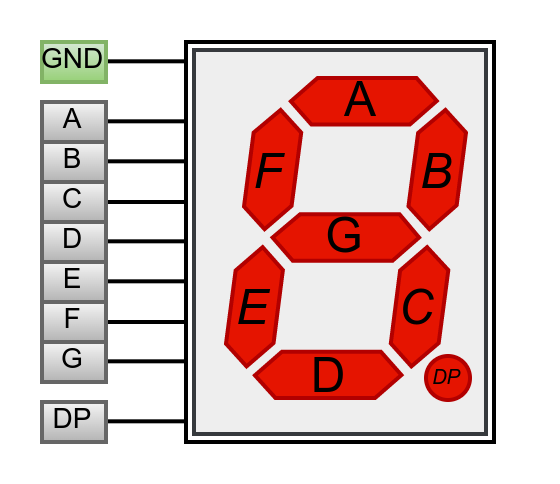
\includegraphics[width=0.39\textwidth]{7SEGMENT.png}
    \caption{Schema van het 7-segmentdisplay met een ``dp'' ($decimal$ $point$) ingang.}
    \label{fig:39110}
\end{figure}
\pagebreak
\subsection{Flip-flop's}
Een flip-flop is een geheugenelement dat in de elektronica wordt toegepast. Deze ``flip-flop'' wordt ook wel een ``bistabiele multivibrator'' genoemd. 
Elke soort flip-flop bestaat uit een bepaalde soort latch met één klokingang. Het input signaal voor de latch zal alleen doorgevoerd worden zodra de flank van de klokingang actief HOOG staat \cite{Flowers1983}. 
In dit verslag wordt er gewerkt met twee soorten flip-flop's, namelijk:
\begin{itemize}
    \item De D-flip-flop, wordt ook wel ``data-flip-flop'' genoemd, is een flip-flop dat een data-ingang D en een klokingang heeft;
    \item De J-K-flip-flop, is vernoemd naar ``Jack-Kilby-flip-flop''. Het is een flip-flop dat een klokingang en twee data-ingangen J en K bevat.
\end{itemize}
Zie hieronder de waarheidstabellen van de D-flip-flop en de J-K-flip-flop:
\begin{figure}[h]
    \begin{minipage}{.5\textwidth}
\begin{displaymath}
    \begin{array}{|c||c|c|c|}
    D & Q & \overline{Q} & Comments\\
    \hline 
    1 & 1 & 0 & SET \\
    0 & 0 & 1 & RESET
  \end{array}
    \end{displaymath}
\end{minipage}
\begin{minipage}{.5\textwidth}
\begin{displaymath}
    \begin{array}{|c|c||c|c|c|}
    J & K & Q & \overline{Q} & Comments\\
    \hline 
    0 & 0 & Q_{0} & \overline{Q_{0}} & No\ change\\
    0 & 1 & 0 & 1 & RESET\\
    1 & 0 & 1 & 0 & SET\\
    1 & 1 & \overline{Q_{0}} & Q_{0} & TOGGLE 
  \end{array}
    \end{displaymath}
\end{minipage}
\end{figure}
\\ 
Flip-flop klok signalen kunnen een positieve of een negatieve flank (edge) hebben. Dit houdt in dat de klokpuls pas wordt doorgevoerd aan het begin (positive edge) of einde (negative edge) van een puls. 
Positive edge klokpulsen worden aangegeven met een pijl omhoog en negative edge klokpulsen worden aangegeven met een pijl omlaag. 
Daarnaast kunnen flip-flop's worden toegepast in veel applicaties zoals in schuifregisters, frequentiedelers, dataopslag, tellers en nog veel meer. 
\begin{figure}[h]
    \centering
    \begin{minipage}{.5\textwidth}
      \centering
      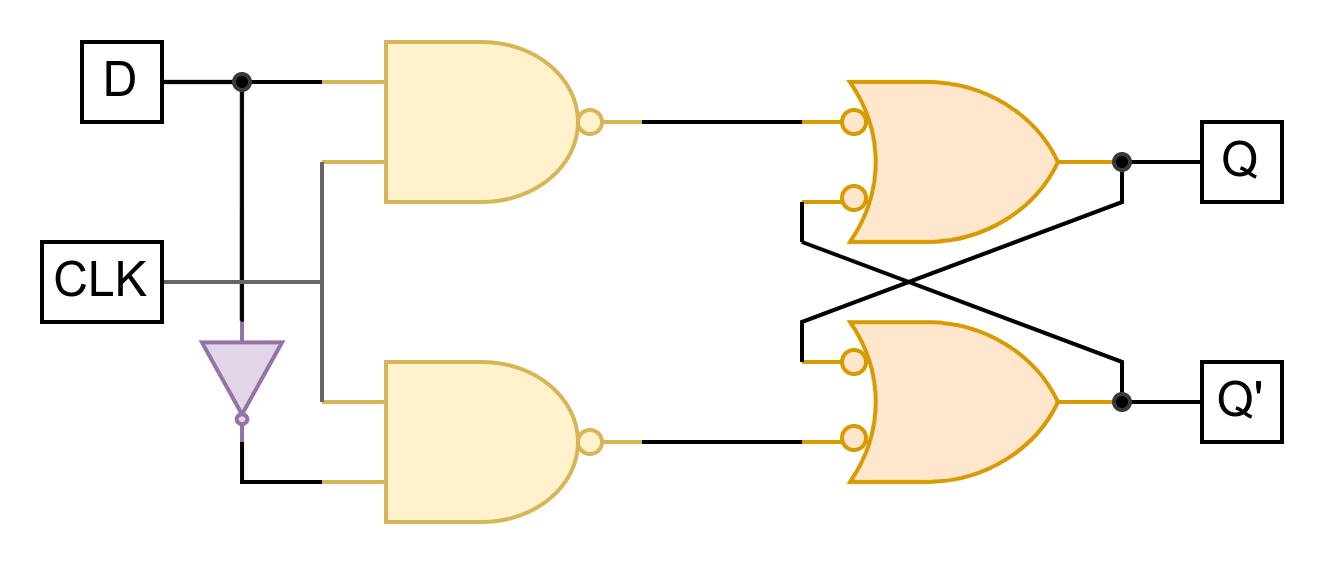
\includegraphics[width=1\linewidth]{dflip.png}
      \caption{Logische schakeling van de D-flip-flop.}
      \label{fig:dflipflop}
    \end{minipage}%
    \begin{minipage}{.5\textwidth}
      \centering
      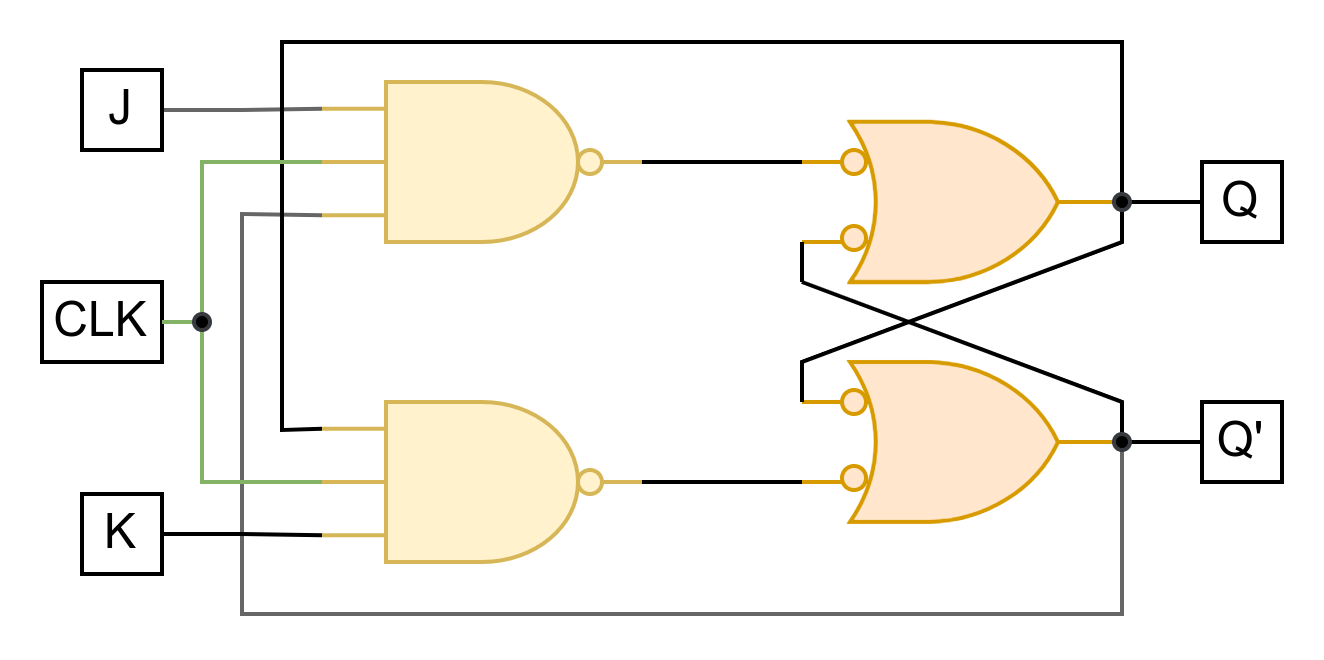
\includegraphics[width=1\linewidth]{jkflip.png}
      \caption{Logische schakeling van de J-K-flip-flop.}
      \label{fig:tessat2}
    \end{minipage}
    \end{figure}
\pagebreak
\subsection{Het 3910 digiboard: versie 2}
De ``Type 3910 DIGI BOARD 2'' is gefabriceerd door \textit{hps SystemTechnik} en is bedoeld als een universele trainingsbord om studenten te laten leren omgaan met logische schakelingen en poorten in de digitale techniek \cite{hps-systemtechnik}. 
Dit digiboard bevat de volgende ingebouwde componenten: \cite{hps-systemtechnik_ds_DIGI}
\begin{enumerate}
    \item 2 input keyboards with 4 pairs of keys (L/H) each;
    \item Clock generator with divider, TTL level, crystal-controlled;
    \item DC signal source 0...5 V/ 10 mA;
    \item Hexadecimal/dual coding switch (double);
    \item LED display, divided into 3 groups with the colors red, yellow, green;
    \item HIGH/LOW, for tapping HIGH, LOW states;
    \item 7-segment display (2-digit), with decoder: dual/7-segment;
    \item Adapter (2 mm jacks/SUB-D socket), for adapting 2 mm jacks to SUB-D connector (25-pin), pins 1...13 and 18 assigned;
    \item 8 AND gates, with pull-up Resistors, one gate is disconnectable;
    \item 6 OR gates, with pull-down Resistors, one gate is disconnectable;
    \item 3 AND/OR combi-gates;
    \item 1-bit comparator;
    \item 4-bit comparator;
    \item 4 J-K-flipflops, can also be used as RS flipflops;
    \item 4 D-flipflops;
    \item 2 adders (4-bit), with input and output carry;
    \item Monoflop, settable times: 0.1s; 1s; 5s;
    \item Multiplexer, 4 channels;
    \item Demultiplexer, 4 channels;
    \item Shift register (4-bit), parallel and serial operation possible, bidirectional;
    \item ALU, for conducting 16 arithmetic and 16 logical computing operations with 4-bit dual numbers;
    \item Binary counter (4-bit), up/down counter;
    \item 2 inverters with open collector (pull-up resistors can be connected);
    \item 2 Schmitt triggers, inverting;
    \item Units complements for negating a 4-bit binary number;
    \item Antivalence and equivalence gates;
    \item RAM 8x4, static RAM, 8 addresses, 4 bits data width;
    \item EEPROM 8x4, storage time without power supply approx. 1 hour;
    \item AD / DA converter (4-bit);
    \item Two slots for expanding a circuit with additional plug-in modules.
\end{enumerate}
Zie de afbeelding hieronder voor de representatie van het digiboard:
\begin{figure}[h]
    \centering
    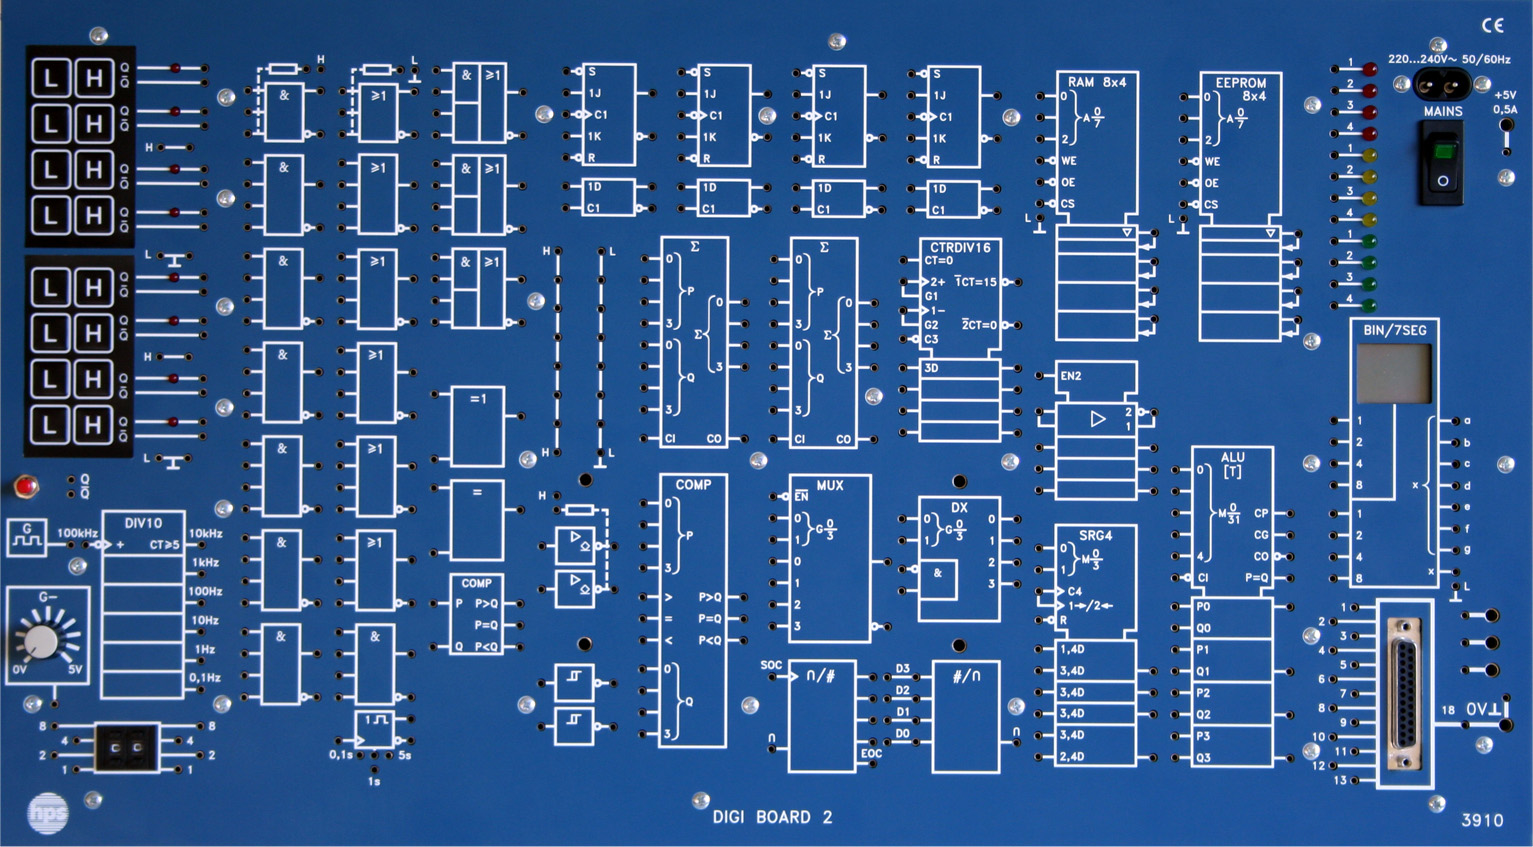
\includegraphics[width=0.8\textwidth]{3910.jpg}
    \caption{Foto van de ``Type 3910 DIGI BOARD 2''.}
    \label{fig:3910}
\end{figure}
\pagebreak
\section{Methode en aanpak}
Om dit practicum op een juiste manier uit te voeren is de volgende methodiek toegepast:\\
1. De voorbereiding voor het practicum:
\begin{itemize}
  \item De practicum benodigdhedenlijst (zie: H\ref{practicumbenodigdheden}) bekijken en de benodigdheden verzamelen en klaarzetten voor gebruik;
  \item Het theoretische kader (zie: H\ref{Theoretisch kader}) van dit verslag even goed doornemen zodat je weet hoe bepaalde materialen en de theorie in elkaar zit;
  \item De vragen van het practicum alvast bekijken en vervolgens zoeken naar mogelijke antwoorden zodat je dat (mogelijk) in ieder geval al klaar hebt staan. 
\end{itemize}
2. Het uitvoeren van het practicum:
\begin{itemize}
    \item Ga rustig door de vragen heen en noteer je antwoorden, als je iets niet weet kun je het altijd nog op internet zoeken of bij de bijbehorende docent een vraag stellen;
    \item Maak foto's van de logische schakelingen die je hebt gebouwd tijdens het practicum. Dit zodat je later in je mogelijke verslag kunt bewijzen dat je er ook echt was en alles werkend hebt gekregen;
    \item Ruim alle geleende spullen van school, zoals het digiboard, IC-board en snoeren weer netjes terug in het lab. Bewaar je antwoorden en gemaakte foto's op een juiste manier, zodat je later netjes een verslag kunt schrijven. 
\end{itemize}
3. Het schrijven van het verslag:
\begin{itemize}
    \item Maak een document voor dit practicum en geef een gepaste naam aan je document;
    \item Zorg ervoor dat je in ieder geval een: voorblad, inhoudsopgave, inleiding, probleemstelling, theoretisch kader, methode, resultaten, conclusie en bronvermeldingen in het verslag hebt staan;
    \item Op het voorblad zet je de naam van het verslag, je eigen naam (met evt. studentennummer erbij) en datum;
    \item In je inleiding schrijf je kort een introductie over het practicum zelf en geef je het algemene doel van het verslag aan;
    \item In het theoretisch kader geef je uitleg over de toegepaste theorie tijdens het practicum, hierbij zijn bronnen erg belangrijk;
    \item In de methode geef je uitleg over hoe je alles hebt aangepakt en uitgewerkt hebt, zodat de lezer het practicum mogelijk zelf zou kunnen uitvoeren;
    \item De resultaten/antwoorden splits je op in secties net zoals de vragen zijn gesteld in het practicum bestand. Deze resultaten werk je netjes uit en zet je de gemaakte foto's en schema's in de bijbehorende vraag;
    \item In de conclusie geef je antwoord op je probleemstelling en gestelde doelen aan de hand van je resultaten en bespreek ook de belangrijke bevindingen die je had tijdens het practicum;
    \item Tenslotte moet je ook bronvermeldingen hebben. Hierin staan alle gebruikte bronnen, zoals datasheets, artikelen, verslagen, literatuur en overige online bronnen. Dit zodat de lezer kan checken waar je bepaalde informatie vandaan hebt gehaald en mogelijk meer kan lezen over de gebruikte informatie.
\end{itemize}
\pagebreak
\section{Modulo-16 teller}
In de eerste opdracht zijn de volgende deelvragen onderzocht en beantwoord over de modulo-16 teller:
\begin{enumerate}
    \item Ontwerp met behulp van J-K-flip-flops een modulo-16 teller;
    \item Stel de waarheidstabel van de modulo-16 teller op;
    \item Bouw de schakeling op het digiboard;
    \item Sluit de uitgang van elke flip-flop aan op een LED;
    \item Sluit op de klokingang van de J-K-flip-flops een blokgolf met een frequentie van 1 Hz aan (gebruik hiervoor de DIV 10 generator die zich op het digiboard bevindt);
    \item Controleer of de schakeling alle toestanden doorloopt.
\end{enumerate}
\pagebreak
\subsection{Ontwerp met behulp van J-K-flip-flops een modulo-16 teller}
Zie het ontwerp hieronder:
\begin{figure}[h]
    \centering
    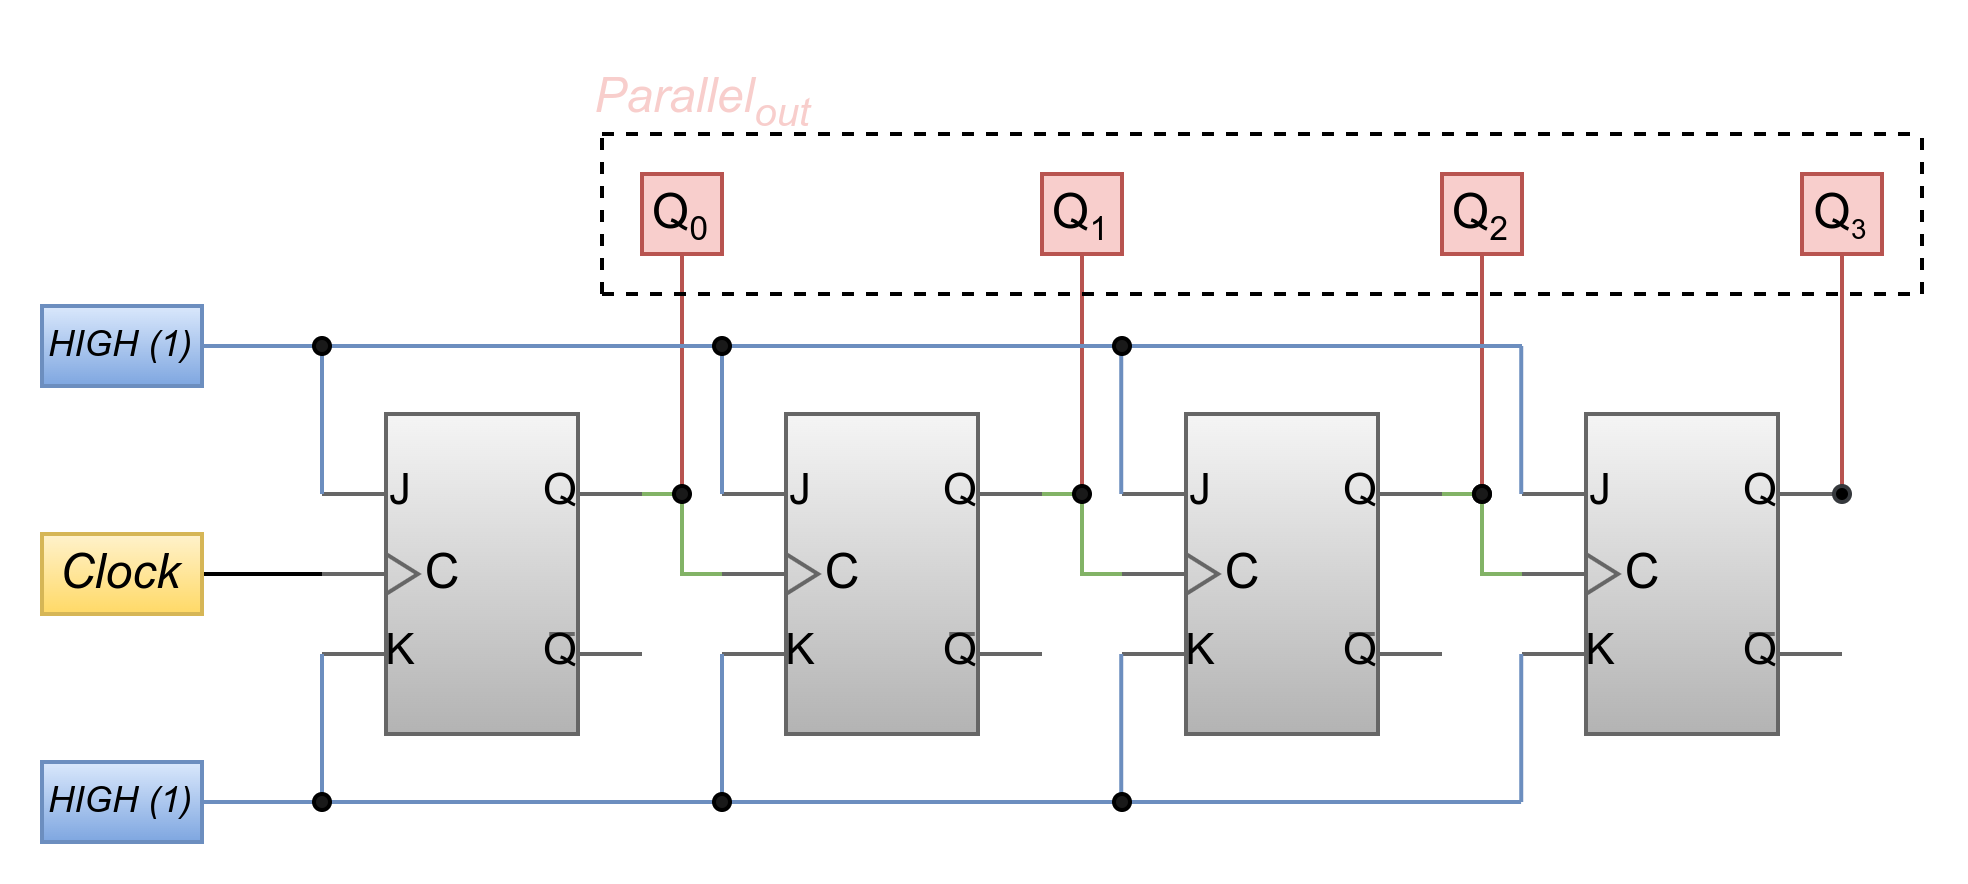
\includegraphics[width=0.8\textwidth]{16mod.png}
    \caption{Logische schakeling dat de modulo-16 teller representeert.}
    \label{fig:16mod}
\end{figure}
\subsection{Stel de waarheidstabel van de modulo-16 teller op}
\label{lol1}
Zie de waarheidstabel van de modulo-16 teller hieronder:
\begin{displaymath}
    \begin{array}{|c||c|c|c|c|}
    CLK & Q_3 & Q_2 & Q_1 & Q_0 \\
    \hline 
    0 & 0 & 0 & 0 & 0 \\
    1 & 0 & 0 & 0 & 1 \\
    2 & 0 & 0 & 1 & 0 \\
    3 & 0 & 0 & 1 & 1 \\
    4 & 0 & 1 & 0 & 0 \\
    5 & 0 & 1 & 0 & 1 \\
    6 & 0 & 1 & 1 & 0 \\
    7 & 0 & 1 & 1 & 1 \\
    8 & 1 & 0 & 0 & 0 \\
    9 & 1 & 0 & 0 & 1 \\
    10 & 1 & 0 & 1 & 0 \\
    11 & 1 & 0 & 1 & 1 \\
    12 & 1 & 1 & 0 & 0 \\
    13 & 1 & 1 & 0 & 1 \\
    14 & 1 & 1 & 1 & 0 \\
    15 & 1 & 1 & 1 & 1 
  \end{array}
    \end{displaymath}
    \pagebreak
\subsection{Bouw de schakeling op het digiboard}
\begin{figure}[h]
    \centering
    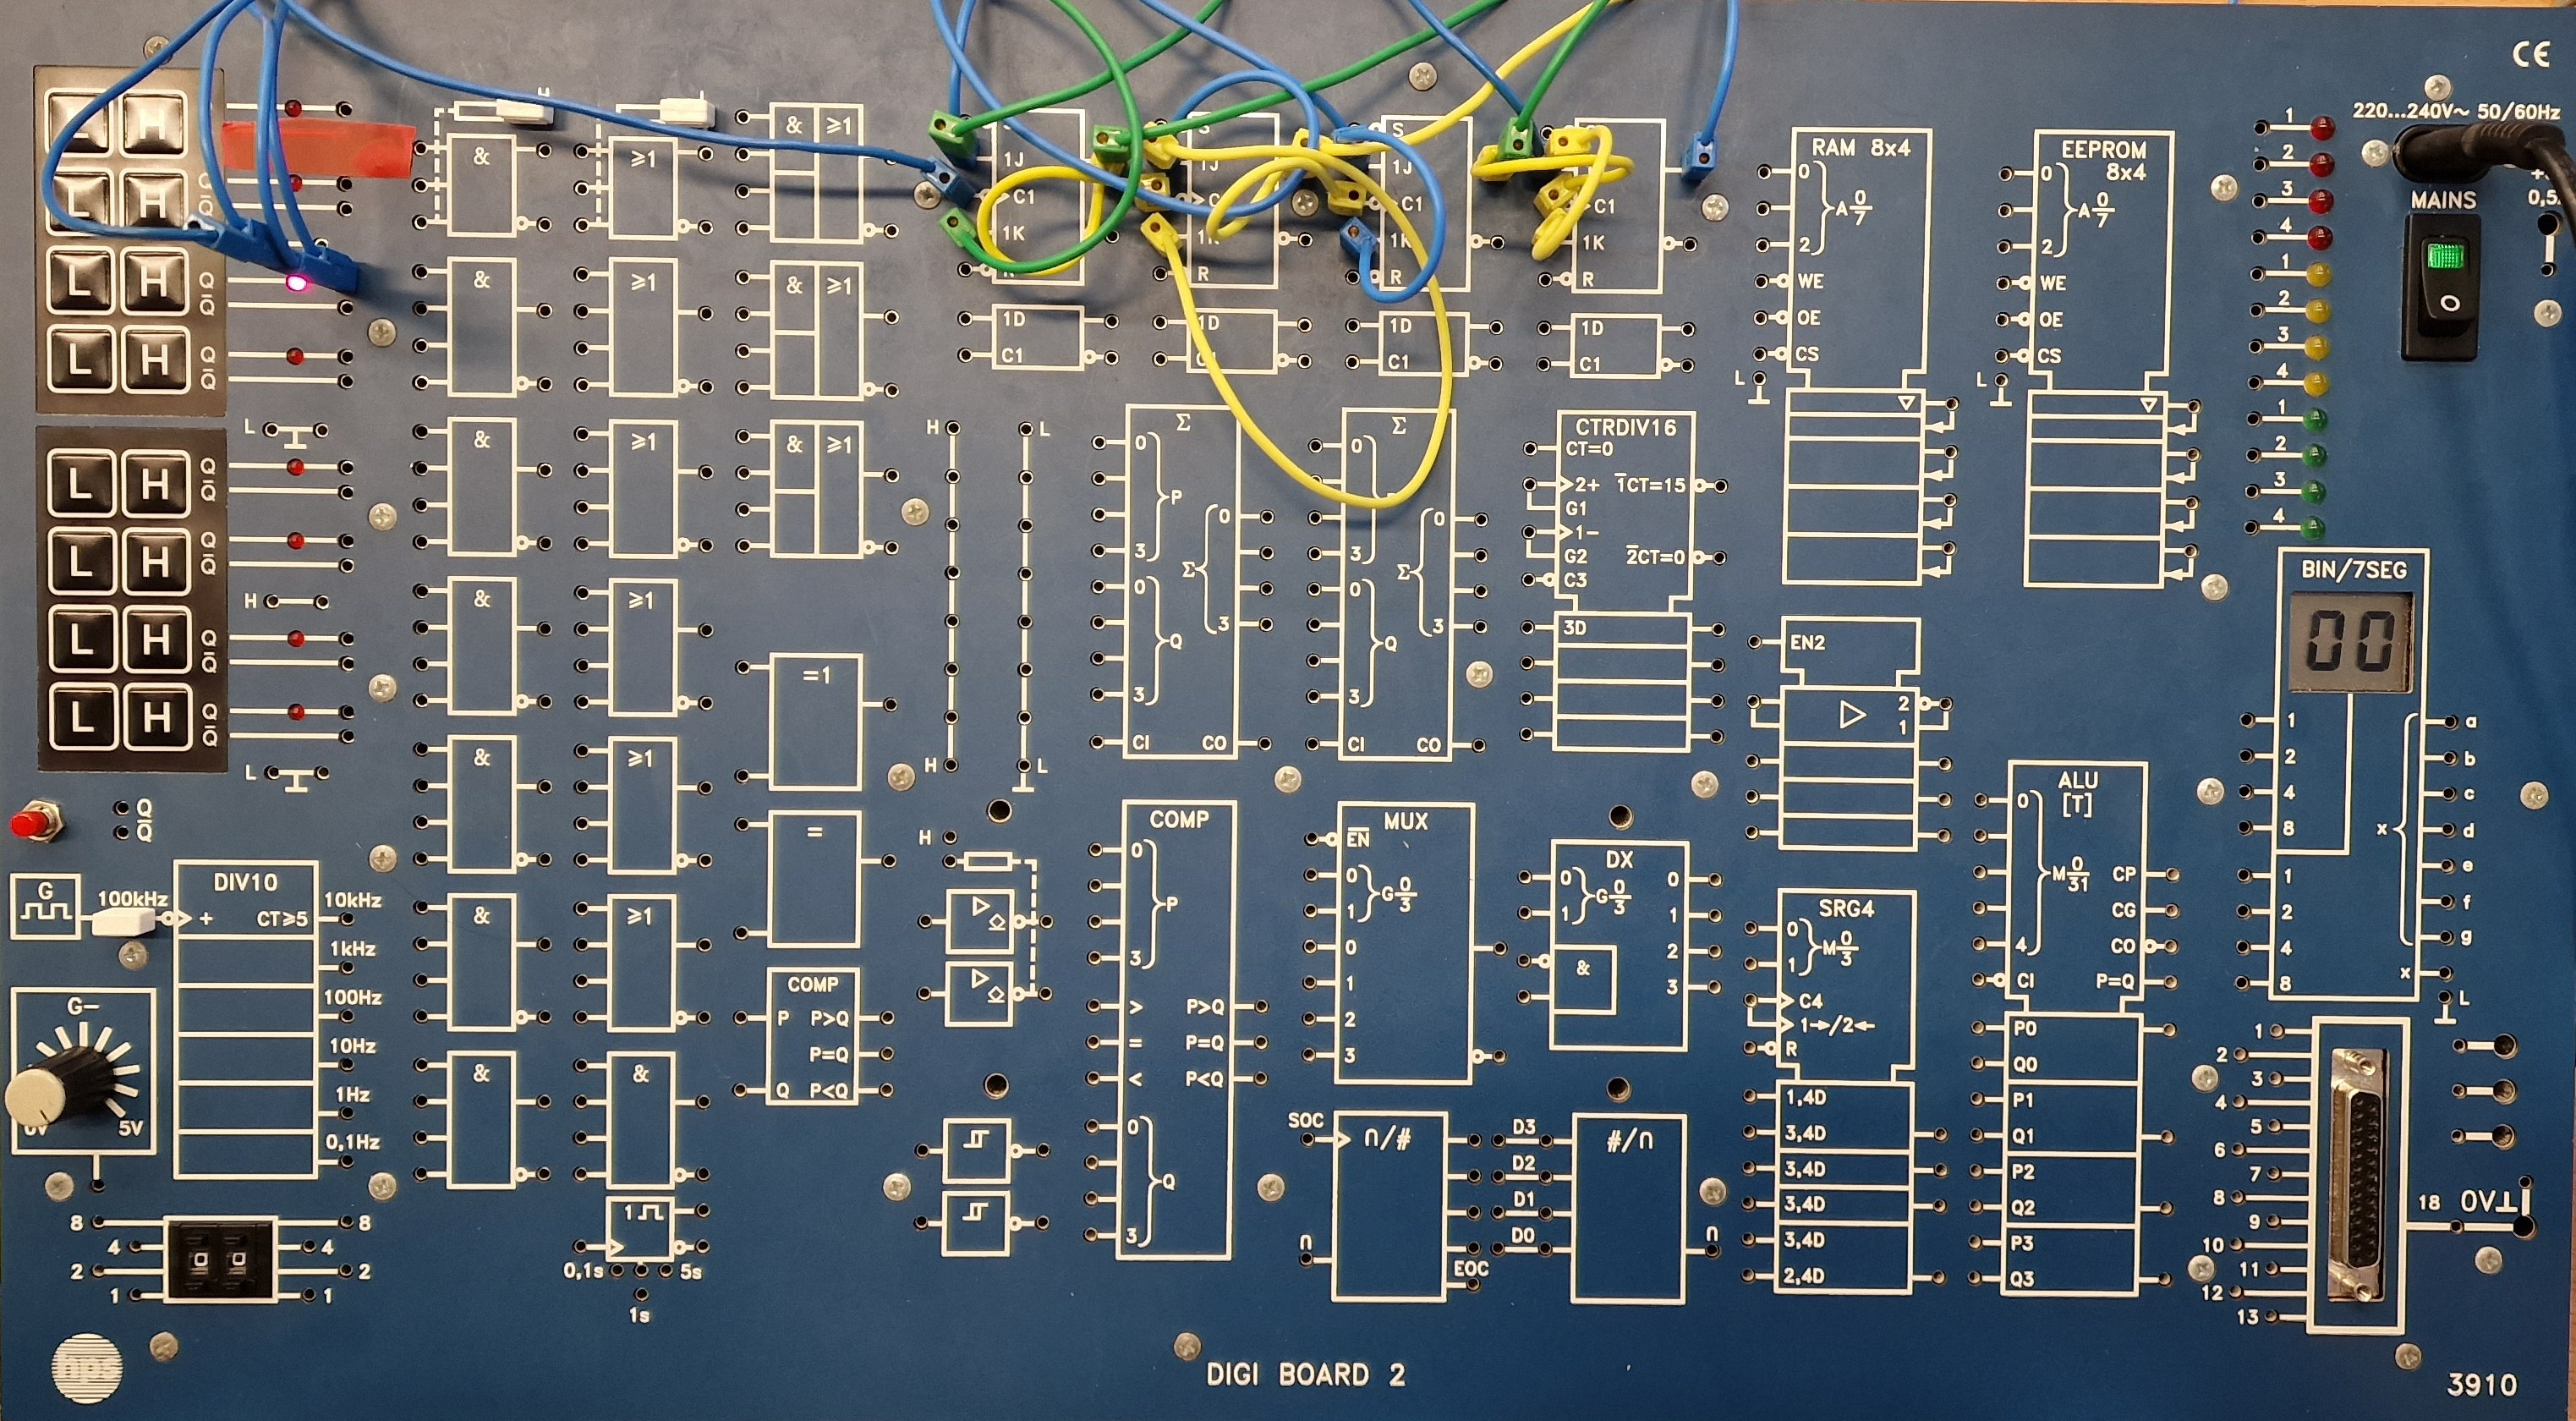
\includegraphics[width=0.75\textwidth]{16LOS.jpg}
    \caption{Gebouwde logische schakeling van de modulo-16 teller.}
    \label{fig:16modg}
\end{figure}
\subsection{Sluit de uitgang van elke flip-flop aan op een LED}
\begin{figure}[h]
    \centering
    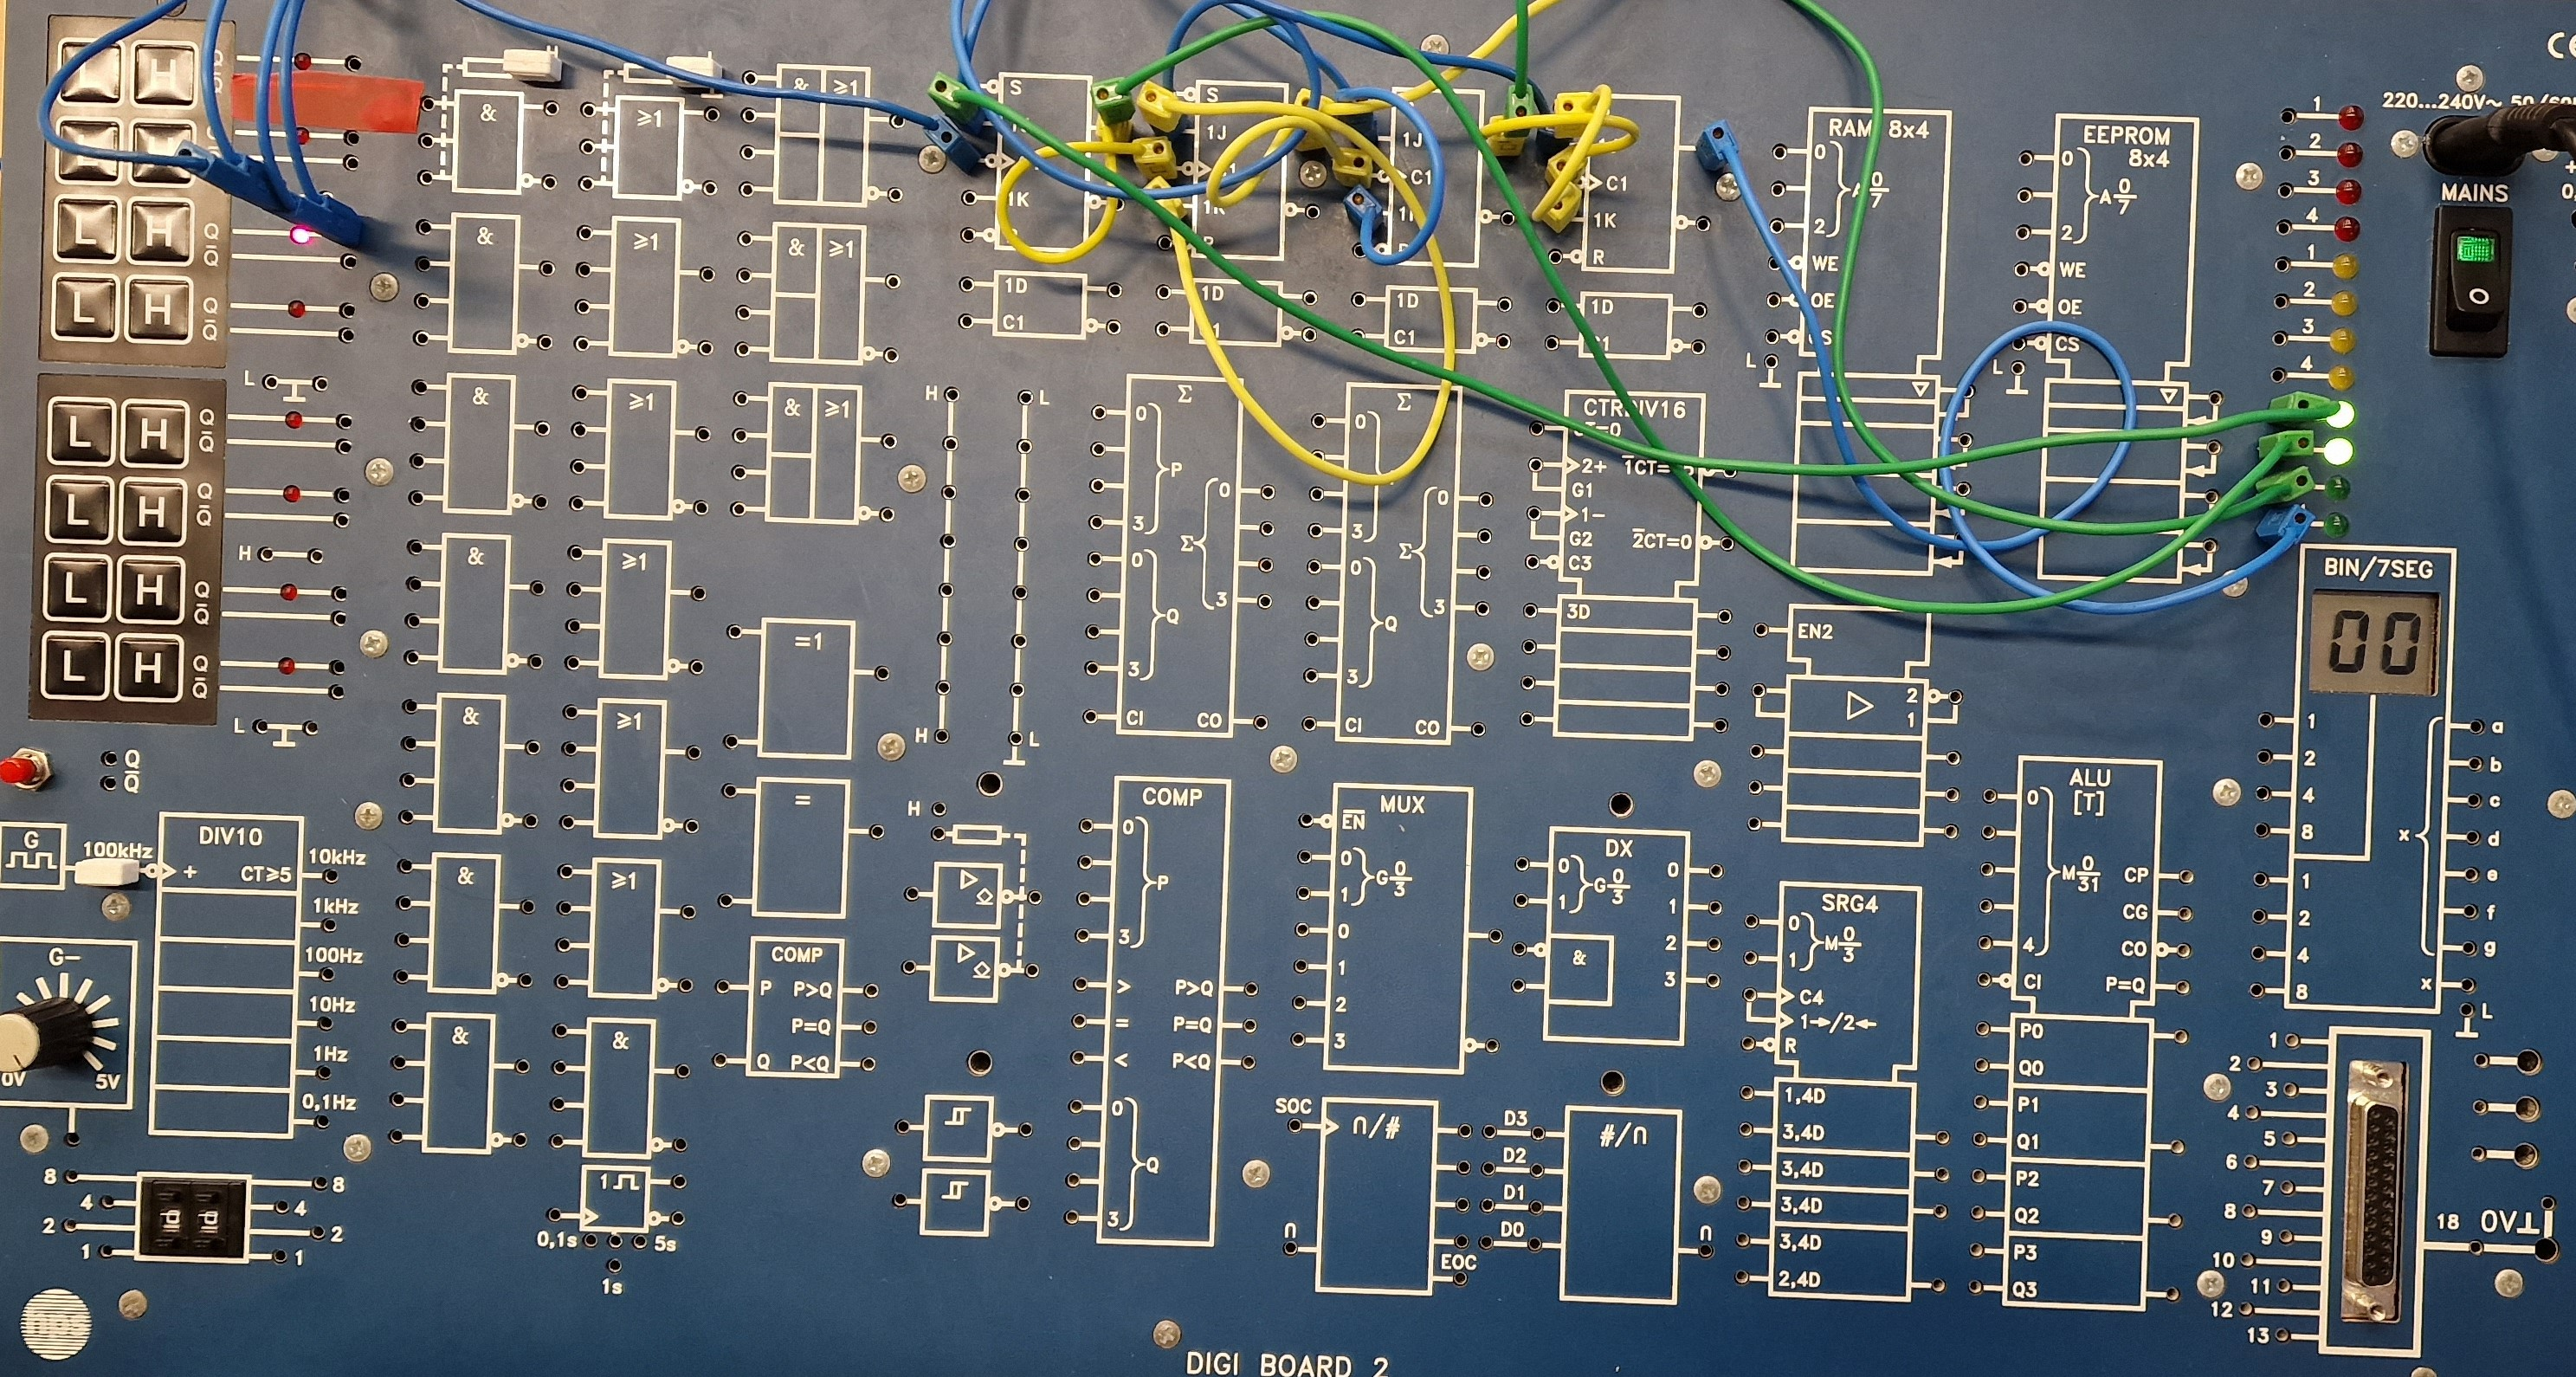
\includegraphics[width=0.75\textwidth]{16LED2.jpg}
    \caption{Gebouwde logische schakeling van de modulo-16 teller.}
    \label{fig:16modgl}
\end{figure}
Hierbij zijn de output snoeren aangesloten aan LED's.
\pagebreak
\subsection{Sluit op de klokingang van de J-K-flip-flops een blokgolf met een frequentie van 1 Hz aan (gebruik hiervoor de DIV 10 generator die zich op het digiboard bevindt)}
\begin{figure}[h]
    \centering
    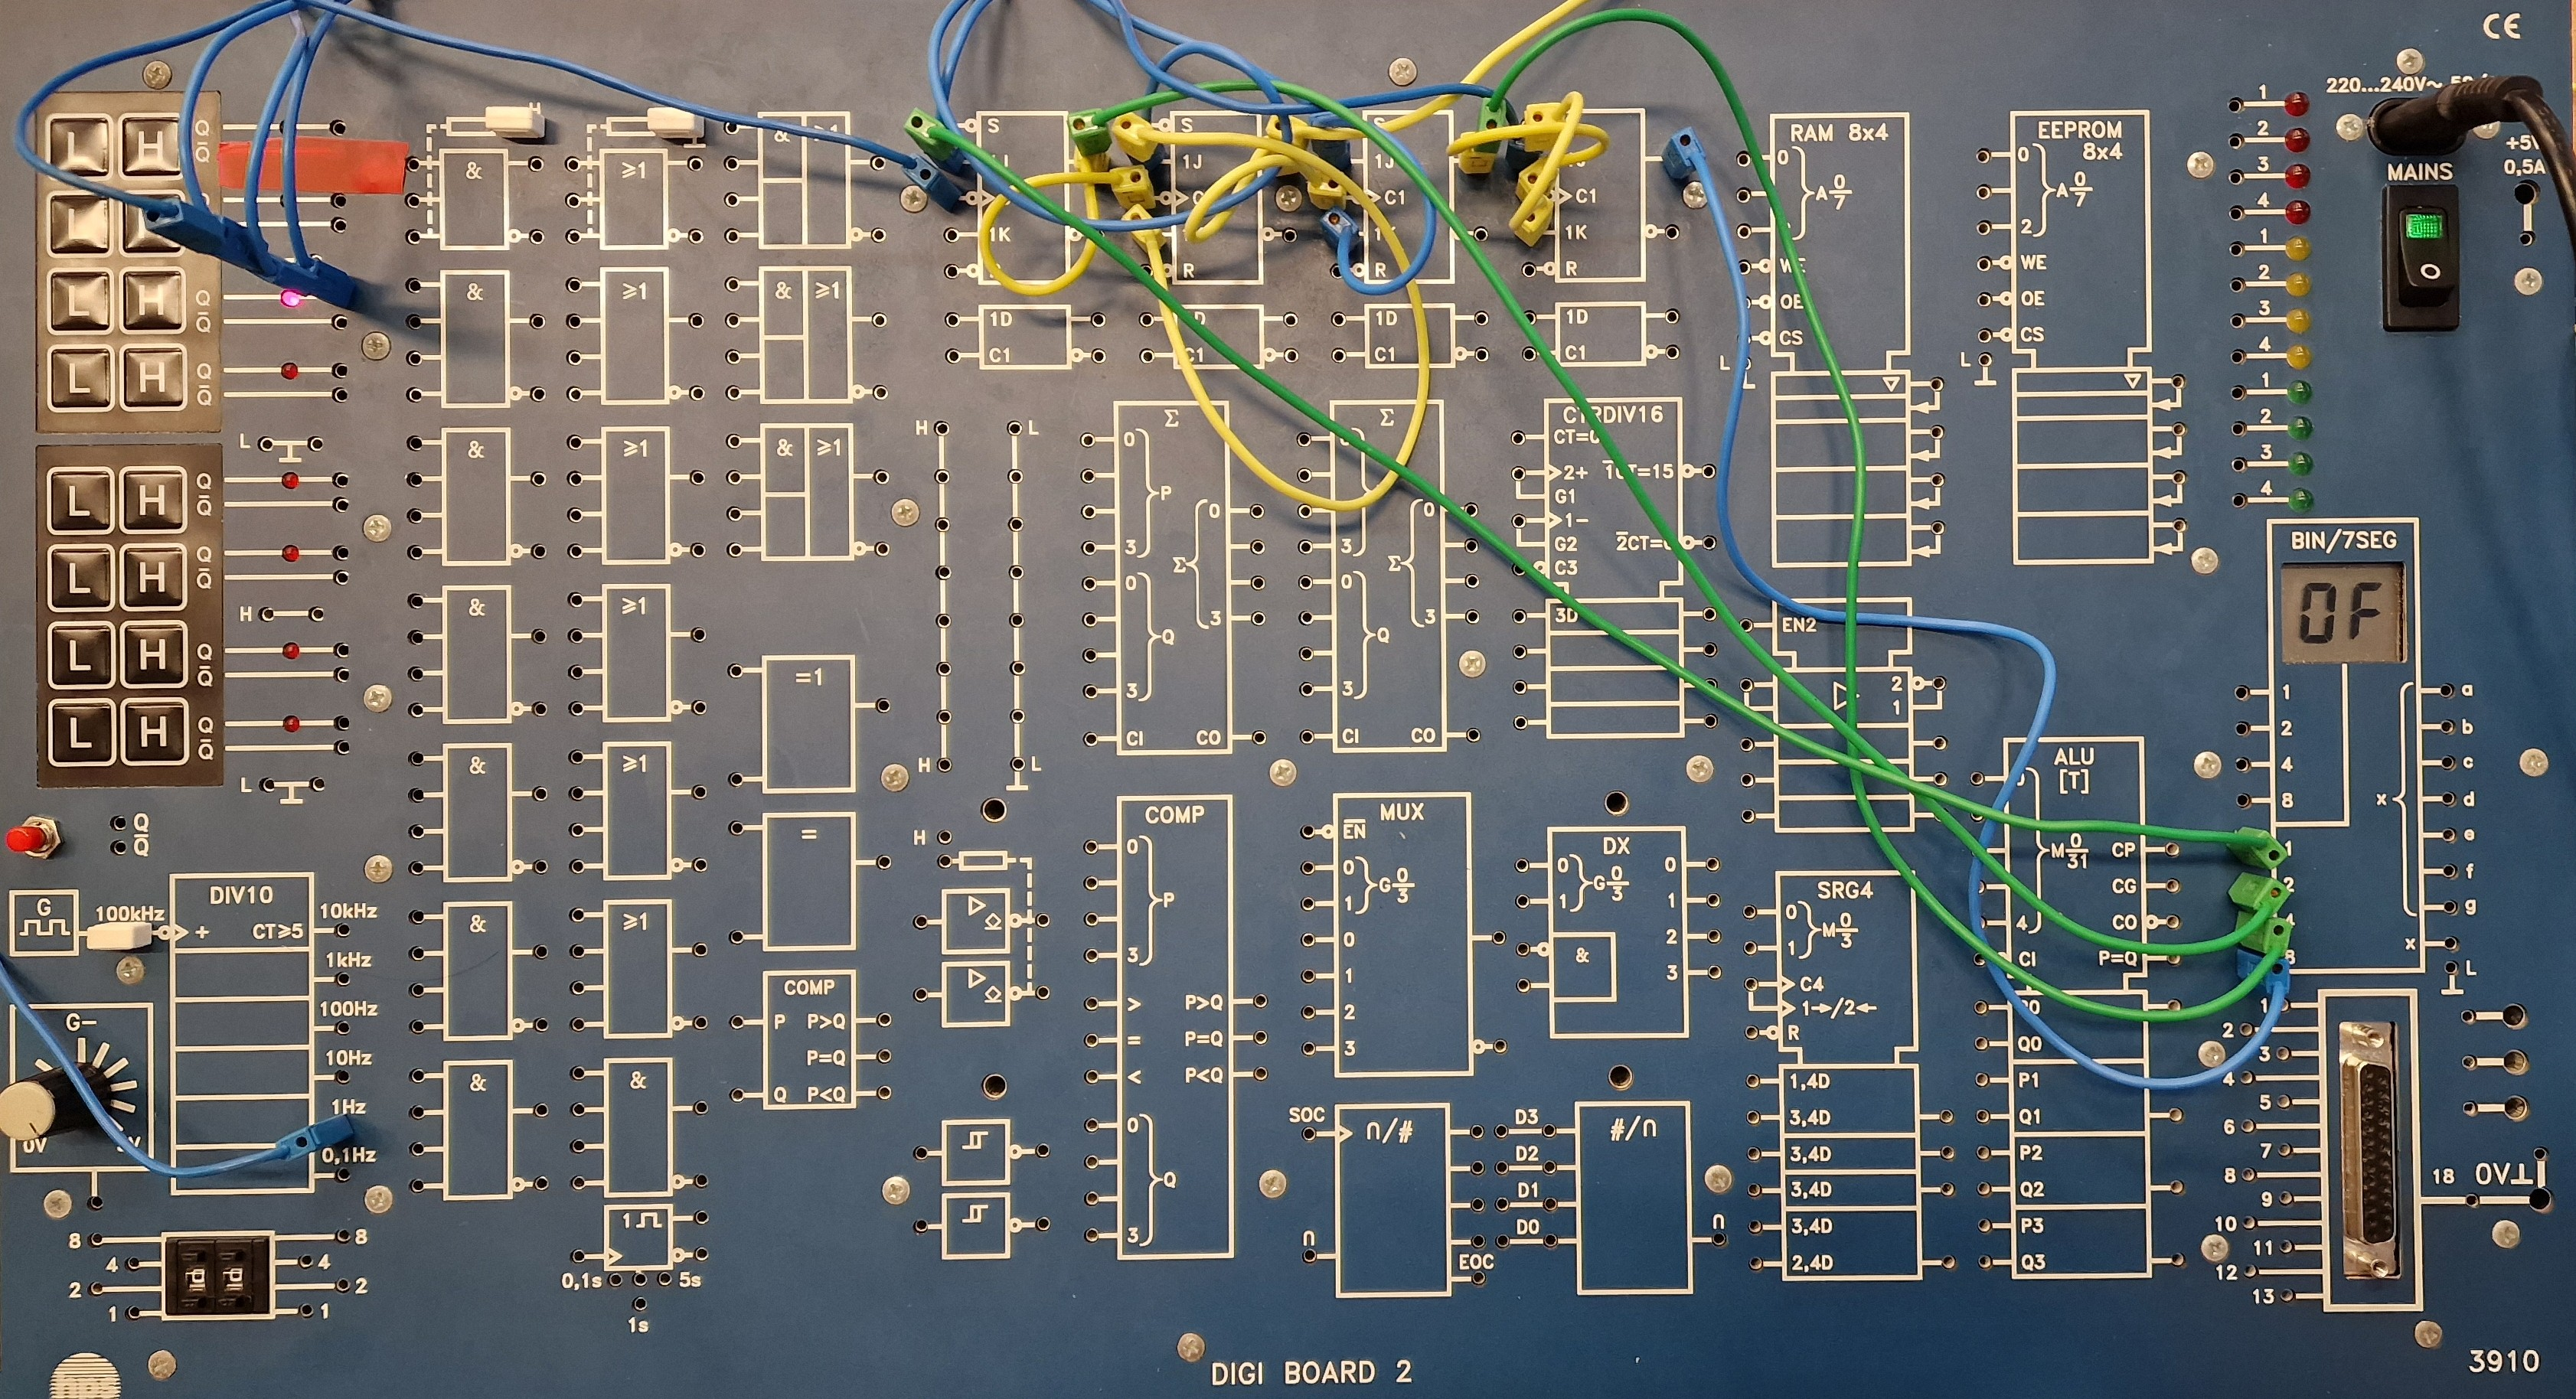
\includegraphics[width=0.8\textwidth]{16SEG.jpg}
    \caption{Gebouwde logische schakeling van de modulo-16 teller.}
    \label{fig:16modg}
\end{figure}
Hierbij zijn de output snoeren aangesloten aan het BIN/7SEG-display van het digiboard. Daarnaast wordt de klokingang gevoed door de DIV10-generator met een frequentie van 1 Hz.
\subsection{Controleer of de schakeling alle toestanden doorloopt}
De gebouwde logische schakeling doorloopt elke toestand, net als in de waarheidstabel in H\ref{lol1}. 
\pagebreak
\section{Decade teller}
\begin{enumerate}
    \item Stel de waarheidstabel van een decade-teller op;
    \item Ontwerp met behulp van J-K-flip-flops een decade-teller (houd er rekening mee dat de teller maar van 0 t/m 9 mag tellen!);
    \item Bouw deze schakeling op het digiboard en sluit de uitgang van elke flip-flop aan op een LED;
    \item Sluit op de klokingang van de J-K-flip-flops een blokgolf met een frequentie van 1 Hz aan (gebruik hiervoor de DIV 10 generator die zich op het digiboard bevindt);
    \item Controleer of de schakeling alle toestanden doorloopt;
    \item Sluit nu de uitgangen van de flip-flops aan op de BCD-uitgangen van de BIN/7SEG decoder (houd rekening met de LSB en MSB!);
    \item Controleer of de schakeling van 0 t/m 9 telt.
\end{enumerate}
\pagebreak
\subsection{Stel de waarheidstabel van een decade-teller op}
\label{lol}
Zie de waarheidstabel van de decade teller hieronder:
\begin{displaymath}
    \begin{array}{|c||c|c|c|c|}
    CLK & Q_3 & Q_2 & Q_1 & Q_0 \\
    \hline 
    0 & 0 & 0 & 0 & 0 \\
    1 & 0 & 0 & 0 & 1 \\
    2 & 0 & 0 & 1 & 0 \\
    3 & 0 & 0 & 1 & 1 \\
    4 & 0 & 1 & 0 & 0 \\
    5 & 0 & 1 & 0 & 1 \\
    6 & 0 & 1 & 1 & 0 \\
    7 & 0 & 1 & 1 & 1 \\
    8 & 1 & 0 & 0 & 0 \\
    9 & 1 & 0 & 0 & 1 
  \end{array}
    \end{displaymath}
\subsection{Ontwerp met behulp van J-K-flip-flops een decade-teller}
\begin{figure}[h]
    \centering
    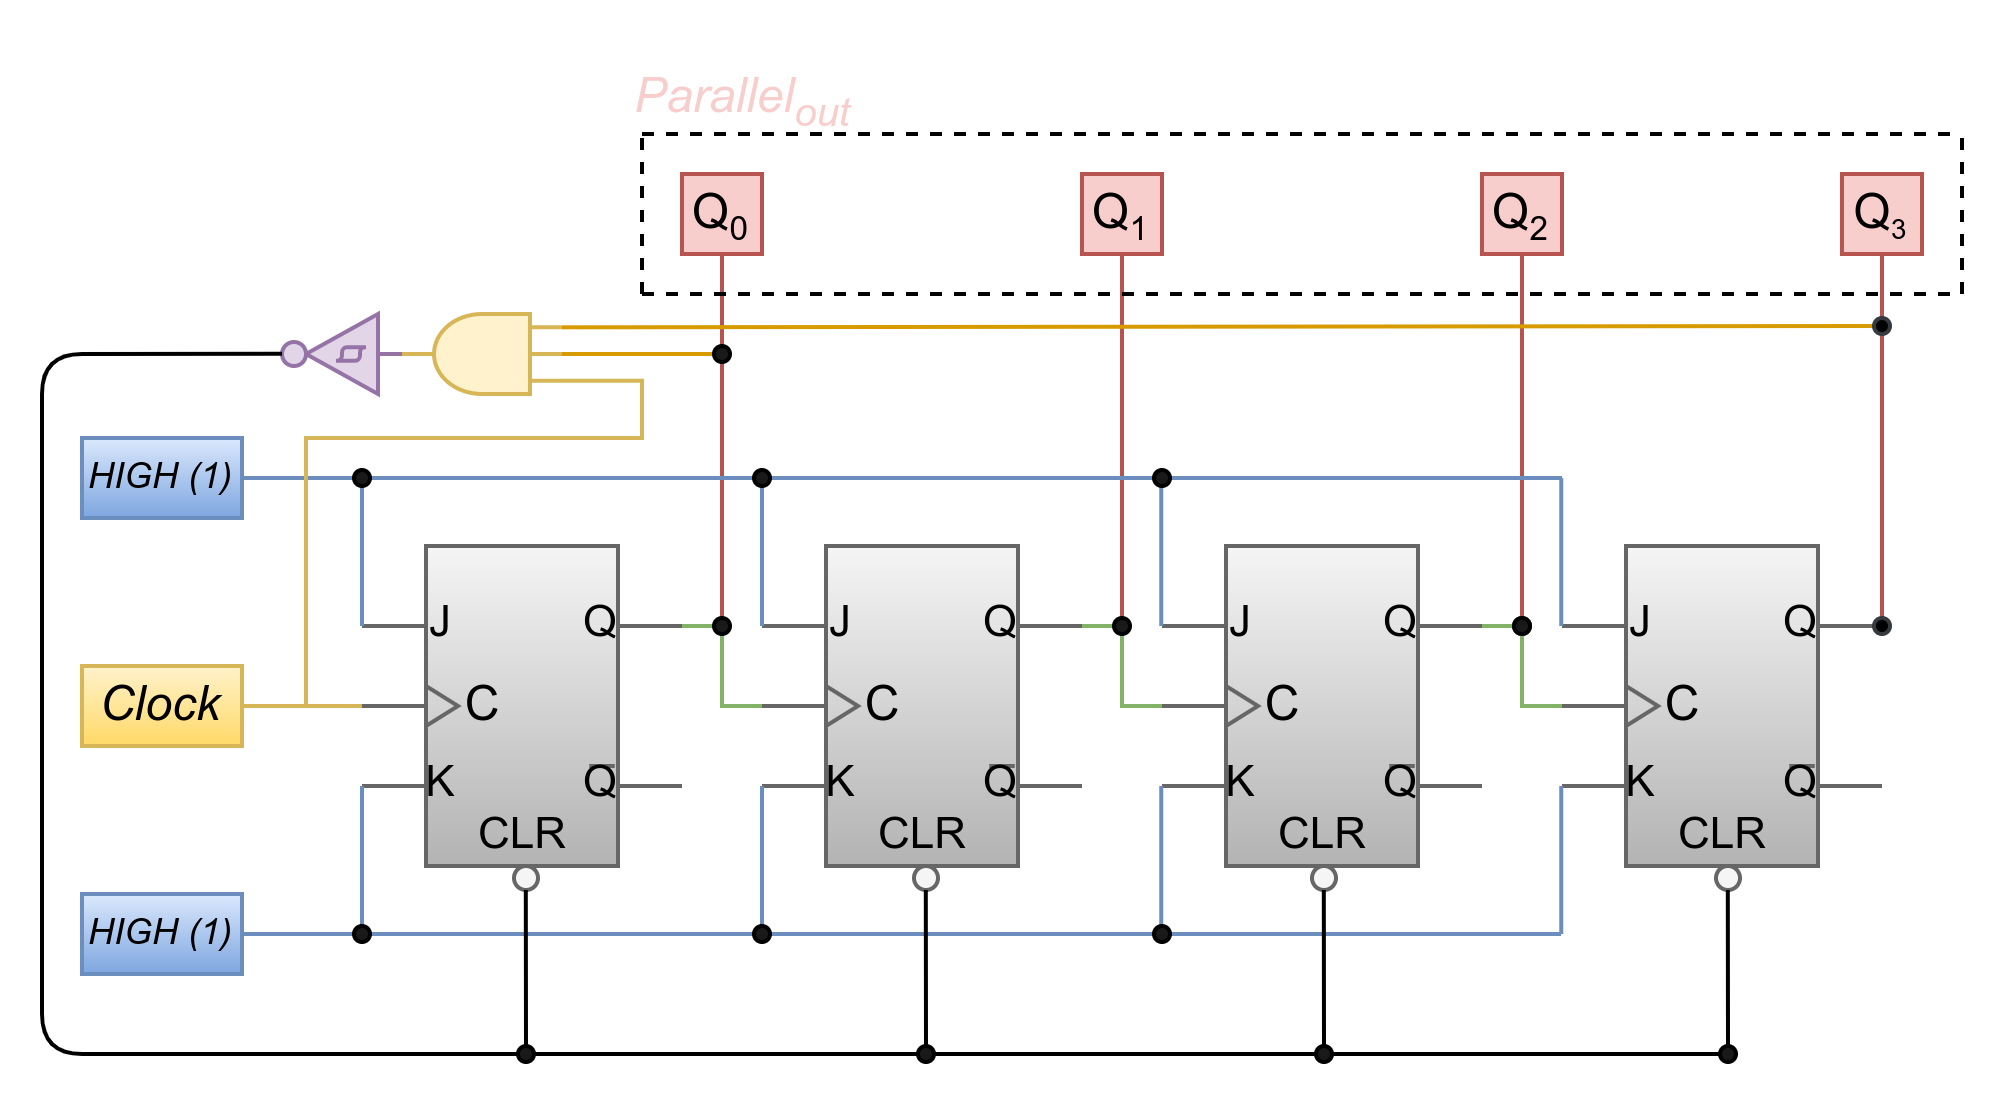
\includegraphics[width=0.8\textwidth]{9mod.png}
    \caption{Logische schakeling van de decade teller.}
    \label{fig:9mod}
\end{figure}
De teller wordt gereset bij het getal 9. Dit is gedaan door gebruik van een AND-poort en een inverted Schmitt-trigger. De AND-gate wordt actief hoog wanneer $1001_2$ en de klokpuls actief hoog zijn.
\pagebreak
\subsection{Bouw deze schakeling op het digiboard en sluit de uitgang van elke flip-flop aan op een LED} 
\begin{figure}[h]
    \centering
    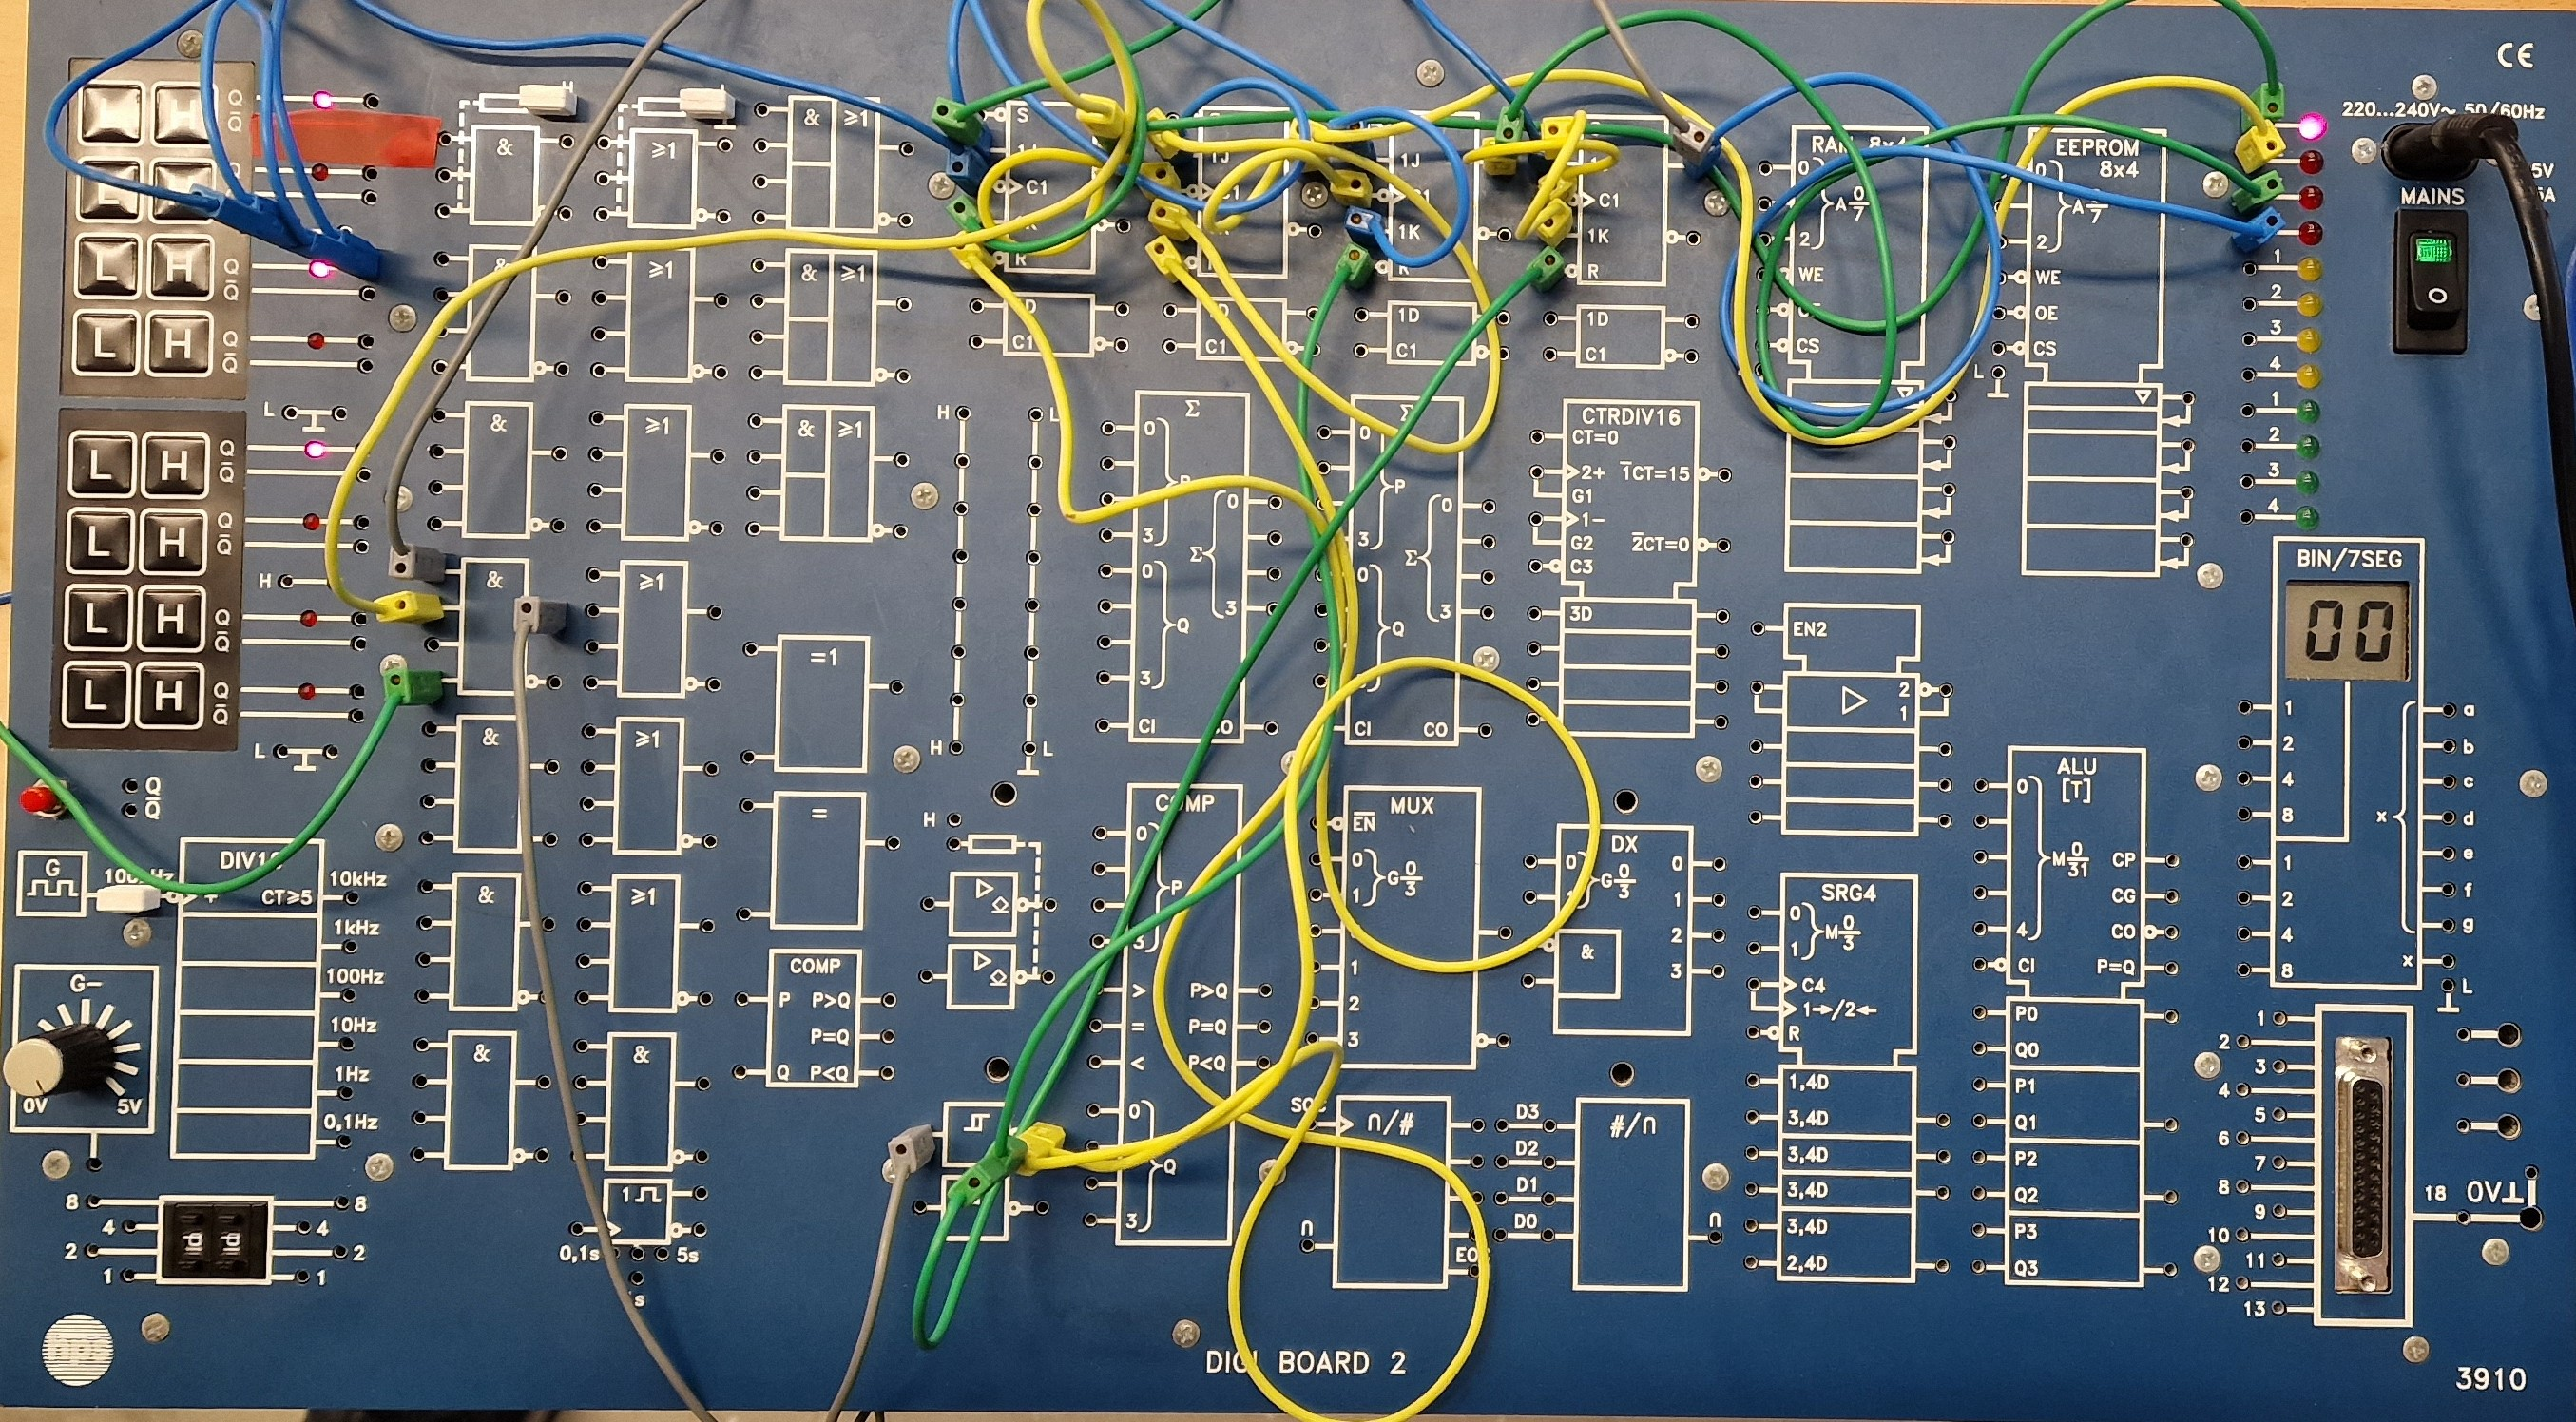
\includegraphics[width=0.7\textwidth]{9LED.jpg}
    \caption{Gebouwde logische schakeling van de decade teller. Hierbij zijn de outputsnoeren verbonden aan LED's }
    \label{fig:9mod}
\end{figure}
\subsection{Sluit op de klokingang van de J-K-flip-flops een blokgolf met een frequentie van 1 Hz aan}
\begin{figure}[h]
    \centering
    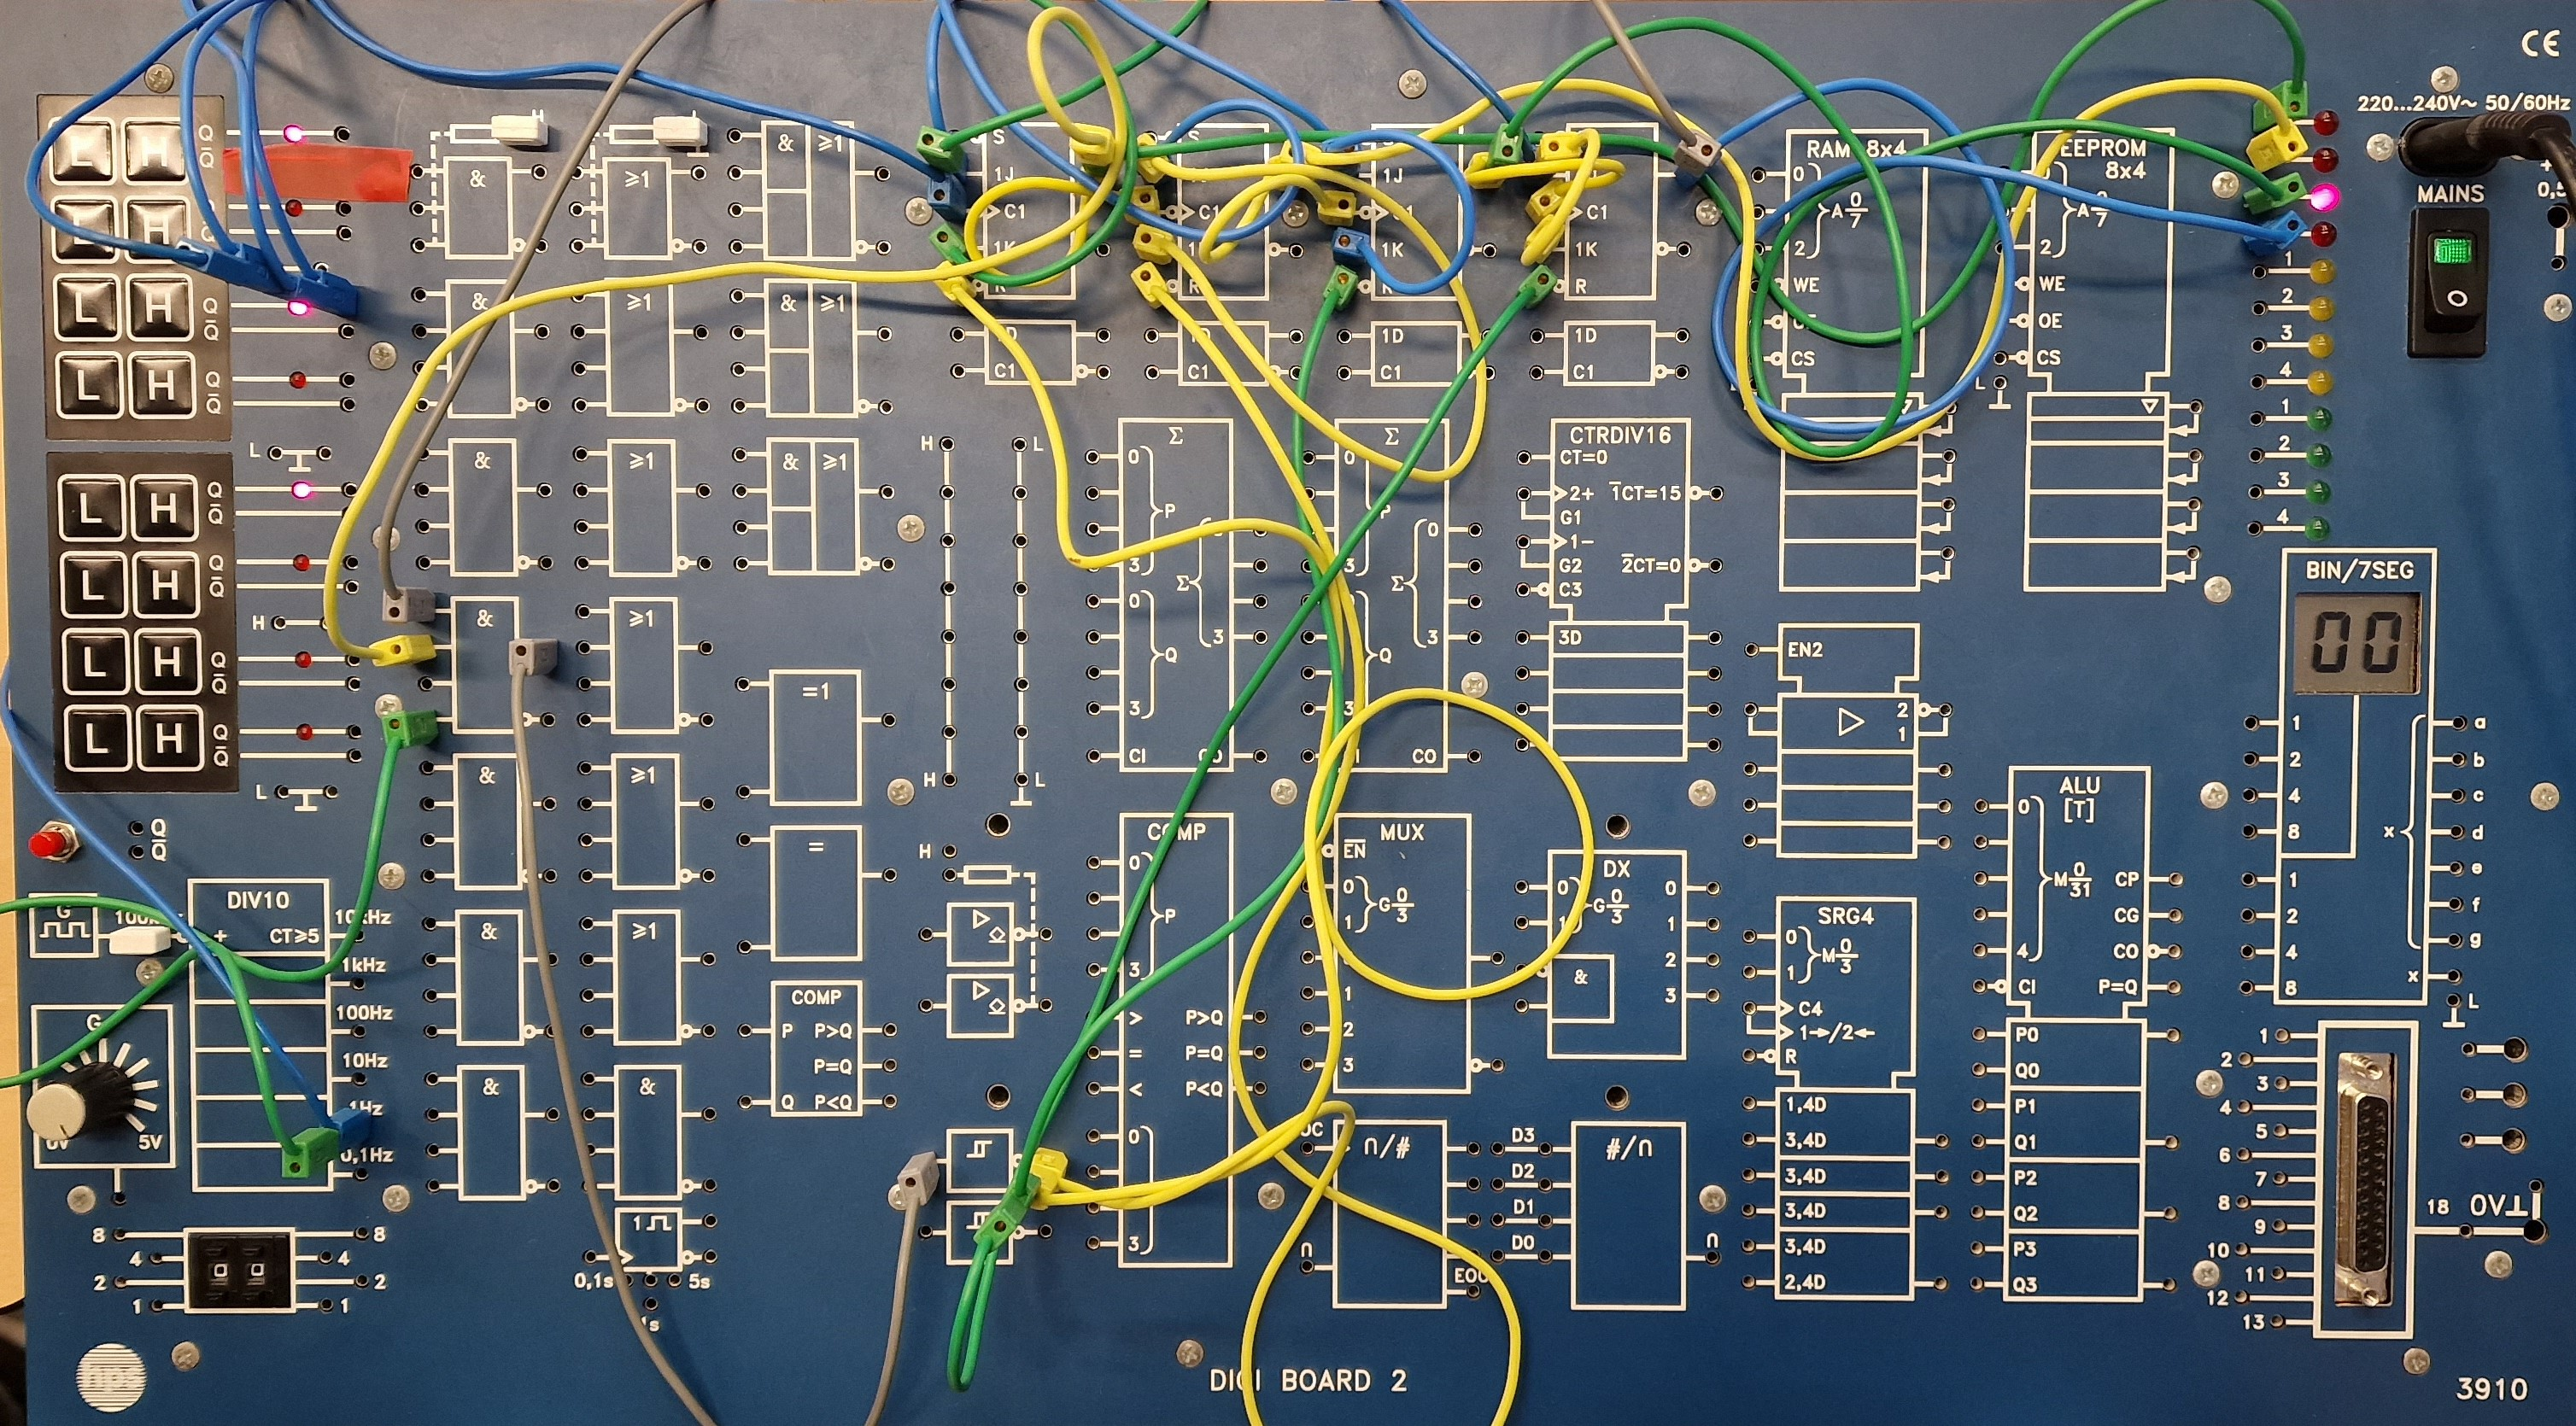
\includegraphics[width=0.7\textwidth]{9LEDCLK.jpg}
    \caption{Gebouwde logische schakeling van de decade teller.}
    \label{fig:9mod}
\end{figure}
Hierbij zijn de outputsnoeren verbonden aan LED's en is de klokingang aangesloten aan de DIV10-klokgenerator.
\pagebreak
\subsection{Controleer of de schakeling alle toestanden doorloopt}
Met succes komen alle toestanden overeen, zoals beschreven is in de decade teller zijn waarheidstabel in H\ref{lol}.
De decade teller begint bij 0 en telt tot en met 9 bij elke klokpuls. 
Zodra de teller bij het getal 9 is, wordt de teller gereset naar 0 en zal het proces zich herhalen. 
\subsection{ Sluit nu de uitgangen van de flip-flops aan op de BCD-uitgangen van de BIN/7SEG decoder}
\begin{figure}[h]
    \centering
    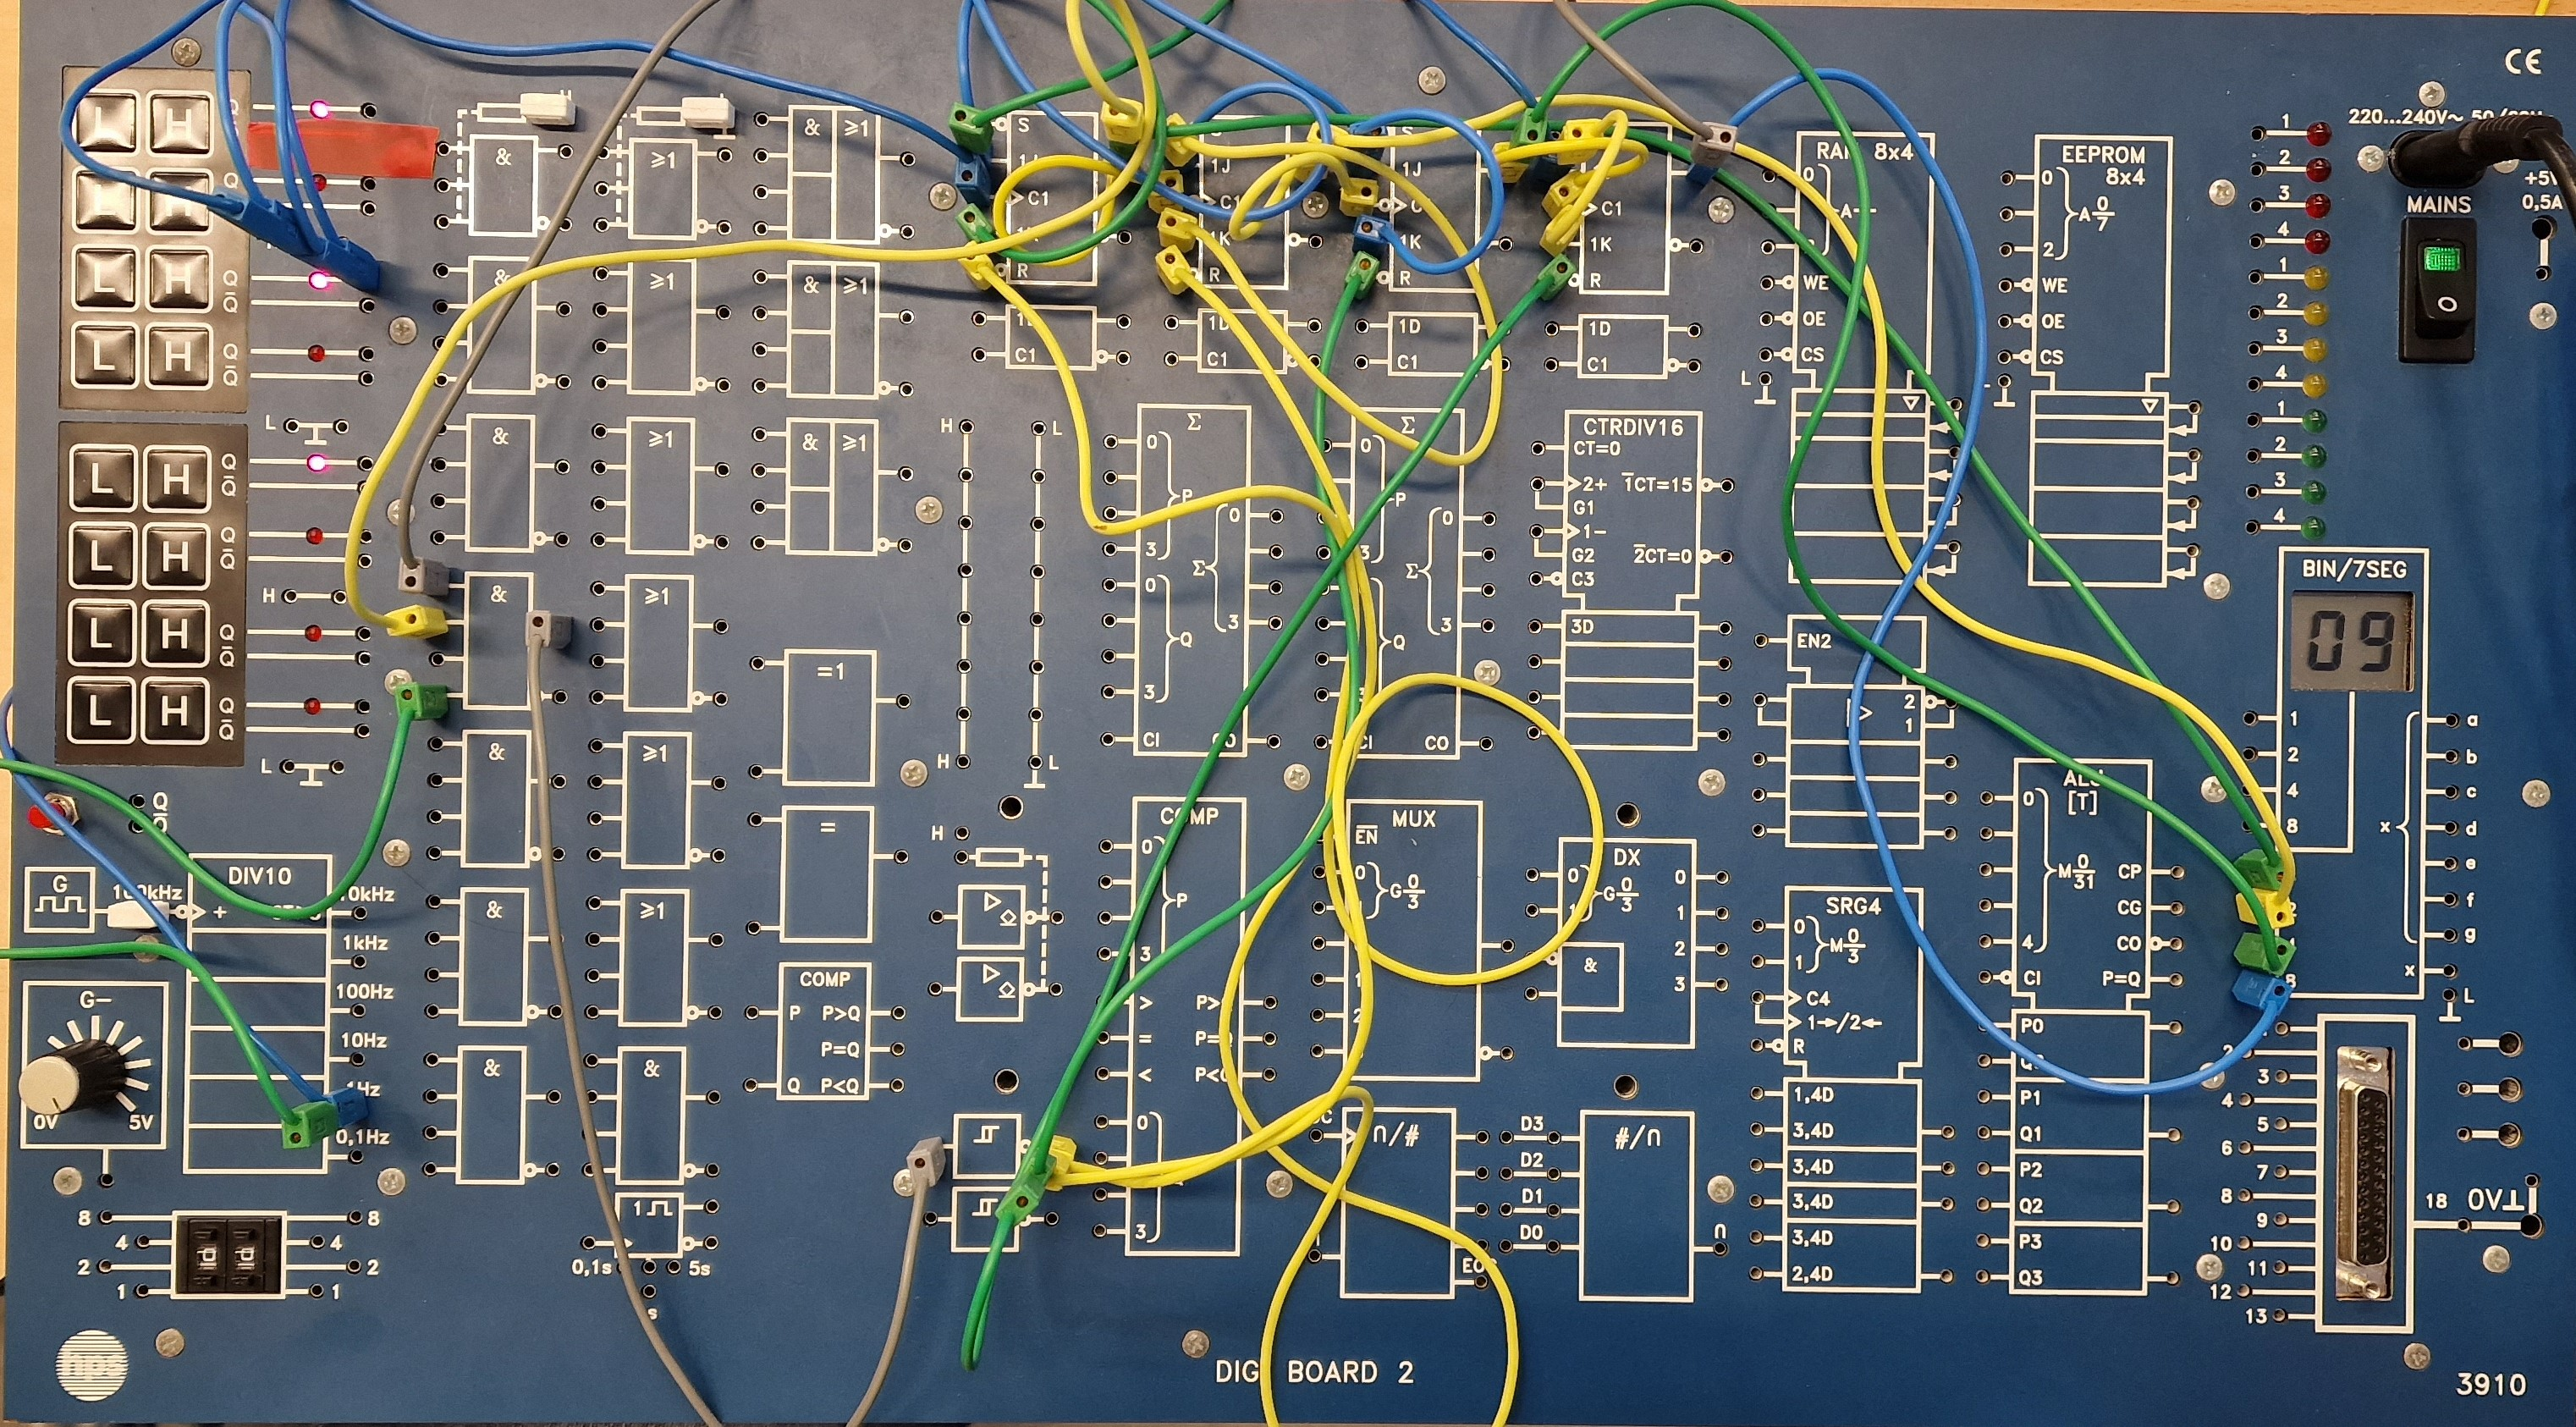
\includegraphics[width=0.7\textwidth]{9SEGCLK.jpg}
    \caption{Logische schakeling van de decade teller.}
    \label{fig:9mod}
\end{figure}

\subsection{Controleer of de schakeling van 0 t/m 9 telt}
Na het aansluiten van de outputsnoeren aan de BIN/7SEG-decoder werkt de decade teller zonder problemen. 
De teller begon bij het getal 0 en telde tot en met het getal 9 met elke klokpuls (1 Hz in dit geval). 
In de foto hierboven is te zien dat de teller bij het getal 9 is, daarna zal de teller terug naar het getal 0 springen en opnieuw beginnen met tellen. 


\pagebreak
\section{Conclusie}
\label{Conclusie}
In dit verslag is er onderzoek gedaan naar de werking van de multiplexer, de BCD-encoder, straight ring counter en de twisted ring counter (Johnson counter). 
Daarbij was ook een probleemstelling geïntroduceerd in H\ref{Problem} en de bijbehorende doelstellingen, zie hieronder:
\begin{enumerate}
    \item Inzicht te verkrijgen in logische functies die ten grondslag liggen aan de digitale techniek;
    \item Waarnemingen te verrichten aan de bijbehorende eenvoudige logische schakelingen;
    \item De bijbehorende meetgegevens en waarheidstabellen op een juiste wijze te verkrijgen en te interpreteren;
    \item De vergaarde gegevens te verwerken tot een verslag.
\end{enumerate}
De probleemstelling was:
\begin{itemize}
    \item \textit{``Hoe kunnen J-K-flip-flops worden toegepast bij het ontwerpen en bouwen van asynchrone tellers?''}
\end{itemize}
 
Bij de eerste practicumopdracht \textit{``Modulo-16 teller''} werd geëxperimenteerd met een asynchrone modulo-16 teller. 
Hierbij was de opdracht om een logische schakeling te ontwerpen en te bouwen dat ervoor zorgt dat er van 0 tot en met 15 geteld kon worden.
Om dat te kunnen doen is er gebruik gemaakt van een waarheidstabel en J-K-flip-flops. 
De bijbehorende logische schakeling is gebouwd, getest en gecontroleerd op de werking ervan en werkte de modulo-16 teller foutloos. 

Vervolgens is er in de tweede practicumopdracht \textit{``Decade teller''} geëxperimenteerd met een asynchrone decade teller. 
Deze decade teller telt van 0 tot en met 9 en dit gebeurt met iedere klokpuls. Zodra de teller bij 9 is, wordt deze gereset naar 0.
De decade teller zal dan dat principe blijven herhalen. 
Tijdens het testen van de logische schakeling werd er in eerste instantie geen inverted Schmitt-trigger gebruikt. 
De decade teller had namelijk alleen een AND-poort met drie ingangen: klokingang, $Q_3$ en $Q_0$. 
Als deze drie ingangen actief hoog zijn, zal de AND-poort een actief hoog signaal geven. 
De teller telde dan tot en met 9, maar wanneer deze gereset werd, sprong de teller naar het getal 2 in plaats van 0. 
Dit komt door onstabiele overgangen in de signalen van de gebruikte logische poorten. 
Logische poorten hebben een maximale stijg en val tijd voor de input, wanneer deze te hoog wordt, kunnen er zulke onstabiele overgangen in signalen ontstaan. 
Er is tijdens het practicum gezocht naar een alternatieve manier. Uiteindelijk werd de inverted Schmitt-trigger uitgeprobeerd, omdat deze werkt met twee spanning-thresholds. 
Door de inverted Schmitt-trigger toe te voegen aan de logische schakeling werkte alles foutloos!
\pagebreak


De bovenstaande probleemstelling is dan ook op een succesvolle wijze opgelost door:
\begin{enumerate}
    \item Eerst te bepalen tot hoog de teller moet gaan met het tellen. Hierbij is het belangrijk om te bepalen hoeveel J-K-flip-flops er nodig zijn;
    \item Daarnaast moet de klokingang alleen aangesloten worden aan de AND-poort en de eerste J-K-flip-flop;
    \item Het aantal AND-poort ingangen is afhankelijk van het maximale telbare getal in het binair. Dat getal moet uiteraard aangesloten worden aan de AND-poort;
    \item De AND-poort moet aangesloten worden aan een inverted Schmitt-trigger, zodat er geen onstabiele signaal overgangen ontstaan;
    \item De output van de inverted Schmitt-trigger moet verbonden zijn met de clear/reset ingang van alle J-K-flip-flops;
    \item Ook moeten alle J en K ingangen van de J-K-flip-flops aangesloten zijn aan een actief hoog signaal;
    \item De output ($Q$) van elk J-K-flip-flop moet aangesloten worden aan de klokingang van de eerst volgende J-K-flip-flop;
    \item Tenslotte is het binaire getal af te lezen als parallelle output. Deze is te vinden in de verbinding tussen elke J-K-flip-flop, inclusief de output ($Q$) van de allerlaatste J-K-flip-flop.
\end{enumerate}
Dus er kan geconcludeerd worden dat de vier doelstellingen van dit practicumverslag met succes gerealiseerd zijn!
\pagebreak






\nocite{*}
\section{Bronvermelding}

\bibliography{library.bib}
\bibliographystyle{IEEEtran}

\pagebreak
\end{document}